% ============================================================
%  BAB 4 — HASIL DAN PEMBAHASAN (REVISI LENGKAP)
% ============================================================
\chapter{HASIL DAN PEMBAHASAN}

Bab ini menyajikan hasil perancangan, pembangunan, dan evaluasi artefak NusaNara
secara komprehensif, mengikuti fase Demonstrasi dan Evaluasi dalam kerangka DSR.

% -------------------------------------------------------
\section{Hasil Perancangan dan Pengembangan Artefak}
% -------------------------------------------------------

\subsection{Pengumpulan Data Kebutuhan Awal}

Pada alur \textit{user-centric}, sebuah survei daring disebarkan untuk dua tujuan utama:
(1) memvalidasi masalah dan tingkat kebingungan karier yang dialami oleh target pengguna,
dan (2) memprioritaskan kebutuhan fungsional sistem sebagai dasar perancangan.
Survei ini berhasil mengumpulkan data dari \textbf{115 responden} yang valid,
yang telah menyetujui \textit{informed consent}.

\subsubsection{Demografi Responden}

Analisis demografi (N=115) menunjukkan bahwa sampel responden sangat relevan dengan
target populasi penelitian. Komposisi jenjang pendidikan, seperti yang divisualisasikan
pada Gambar \ref{fig:demografi}, didominasi oleh Mahasiswa (43,5\%), diikuti oleh
SMA (29,6\%), dan SMK (27\%).

\begin{figure}[H]
  \centering
  
\includegraphics[width=0.75\textwidth]{gambar_4_1_demografi}
  \caption{Diagram Komposisi Jenjang Pendidikan Responden (N=115)}
  \label{fig:demografi}
\end{figure}

Temuan ini diperkuat dengan data sebaran fase pendidikan yang menunjukkan bahwa mayoritas
responden berada pada fase transisi kritis (Gambar \ref{fig:fase}). Data menunjukkan
50\% siswa SMA berasal dari Kelas 12, 45,2\% siswa SMK dari Kelas 11, dan 41,7\%
mahasiswa berasal dari Semester 7 atau lebih. Hal ini mengindikasikan bahwa responden
adalah individu yang sedang aktif menghadapi keputusan karier pasca-kelulusan.

\begin{figure}[H]
  \centering
  
\includegraphics[width=0.90\textwidth]{gambar_4_2_fase}
  \caption{Diagram Sebaran Fase Pendidikan Responden per Jenjang}
  \label{fig:fase}
\end{figure}

Sebaran wilayah responden (Gambar \ref{fig:provinsi}) menunjukkan dominasi dari
Jawa Barat (32,2\%) dan DKI Jakarta (30,4\%), namun terdapat pula responden dari
Bengkulu, Kalimantan Timur, dan Maluku -- menunjukkan jangkauan data yang representatif.

\begin{figure}[H]
  \centering
  
\includegraphics[width=0.75\textwidth]{gambar_4_3_provinsi}
  \caption{Diagram Sebaran 5 Provinsi Teratas Responden}
  \label{fig:provinsi}
\end{figure}

\subsubsection{Validasi Masalah dan Identifikasi Kebutuhan}

Hasil analisis rata-rata skor Likert (skala 1--5) dari tiga aspek utama diringkas
pada Tabel \ref{tab:survei_ringkasan}.

\begin{table}[H]
\centering
\caption{Ringkasan Hasil Analisis Kebutuhan (N=115)}
\label{tab:survei_ringkasan}
\begin{tabularx}{\textwidth}{Xcccc}
\toprule
\textbf{Aspek yang Diukur} & \textbf{Mean} & \textbf{Tingkat} & \textbf{\% Setuju} & \textbf{Interpretasi} \\
\midrule
Tingkat Kecemasan Karier & 4,37 & Tinggi & 92,2\% & Urgensi masalah tervalidasi \\
Evaluasi Layanan Saat Ini & 4,16 & Tinggi & 84,3\% & Kesenjangan solusi signifikan \\
Kebutuhan Sistem Baru     & 4,25 & Tinggi & 87,8\% & Demand kuat untuk sistem baru \\
\bottomrule
\end{tabularx}
\end{table}

Distribusi jawaban Tingkat Kecemasan Karier (Mean 4,37) divisualisasikan pada
Gambar \ref{fig:kecemasan}: 97,4\% responden setuju ``Cemas Salah Jurusan'',
85,4\% ``Khawatir Skill Mismatch'', dan 91,3\% ``Sulit Ambil Keputusan''.

\begin{figure}[H]
  \centering
  
\includegraphics[width=0.90\textwidth]{gambar_4_4_kecemasan}
  \caption{Persentase Tingkat Kecemasan dan Kesulitan Karier (N=115)}
  \label{fig:kecemasan}
\end{figure}

Gambar \ref{fig:layanan} menunjukkan penilaian kritis terhadap layanan yang ada:
91,3\% menyatakan tes minat bakat konvensional kurang menggambarkan diri mereka,
83,5\% merasa layanan kurang interaktif, dan 78,3\% kesulitan menemukan informasi
karier yang relevan dengan konteks lokal Indonesia.

\begin{figure}[H]
  \centering
  
\includegraphics[width=0.90\textwidth]{gambar_4_5_layanan}
  \caption{Persentase Penilaian Terhadap Layanan Karier Saat Ini (N=115)}
  \label{fig:layanan}
\end{figure}

Gambar \ref{fig:kebutuhan} menunjukkan permintaan kuat terhadap sistem baru (Mean 4,25):
85,2\% akan lebih terbantu dengan sistem berbasis narasi, 90,5\% membutuhkan sistem
adaptif, dan 87,9\% menginginkan rekomendasi dalam bentuk narasi langkah-langkah.

\begin{figure}[H]
  \centering
  
\includegraphics[width=0.90\textwidth]{gambar_4_6_kebutuhan}
  \caption{Distribusi Jawaban Kebutuhan Sistem Bimbingan Karier Baru}
  \label{fig:kebutuhan}
\end{figure}

Temuan survei N=115 ini memberikan landasan empiris yang kuat: (1) \textbf{Validasi Masalah}
-- kecemasan karier tinggi (Mean 4,37); (2) \textbf{Kesenjangan Solusi} -- layanan
konvensional dievaluasi kritis (Mean 4,16); dan (3) \textbf{Validasi Solusi} -- demand
kuat terhadap sistem naratif adaptif (Mean 4,25). Ini menjadi dasar konseptual bagi
pengembangan artefak NusaNara.

\subsection{Pengumpulan dan Persiapan Data Lowongan}

\subsubsection{Proses Web Scraping}
Pengumpulan data lowongan dilakukan melalui serangkaian tahapan teknis menggunakan
otomasi Selenium. Evaluasi awal terhadap tiga platform karier utama menghasilkan temuan:

\begin{itemize}[noitemsep]
  \item \textbf{Jobstreet:} proteksi \textit{bot-detection} berbasis Cloudflare memblokir
    permintaan otomatis secara konsisten.
  \item \textbf{LinkedIn:} tidak menampilkan informasi gaji secara publik.
  \item \textbf{Glints:} aksesibel secara teknis dan menyediakan atribut data yang lengkap.
\end{itemize}

Berdasarkan evaluasi ini, Glints dipilih sebagai satu-satunya sumber data. Scraping
menggunakan Selenium WebDriver dengan konfigurasi \textit{selenium-stealth} untuk
menangani konten berbasis JavaScript (SPA).

\subsubsection{Hasil Pengumpulan Data}
Hasil pengumpulan data menghasilkan 720 lowongan pekerjaan yang terdistribusi secara
seimbang ke dalam 8 klaster karier (masing-masing 90 lowongan). Rincian distribusi klaster
telah disajikan pada Tabel \ref{tab:klaster}. Keseimbangan distribusi ini merupakan
persyaratan metodologis yang disengaja agar metrik evaluasi per klaster dapat
dibandingkan secara adil, karena klaster dengan lebih banyak data berpotensi
menghasilkan skor yang lebih tinggi secara inheren \cite{Cormack2009}.



\subsubsection{Hasil Pembersihan Data dan Embedding Vektor (ETL)}
Setelah data mentah berhasil dikumpulkan, proses \textit{Data Cleaning} dan \textit{Embedding} (seperti yang dirancang pada Bab 3) dieksekusi secara berurutan. Hasil dari eksekusi pipeline ETL ini adalah sebagai berikut:

\begin{enumerate}[noitemsep]
  \item \textbf{Hasil \textit{Data Cleaning}:} Dari total 720 dokumen mentah awal, seluruh dokumen (100\%) berhasil dipertahankan. Proses validasi kelengkapan tidak menggugurkan satu pun dokumen karena mekanisme \textit{scraper} sejak awal telah diprogram ketat untuk hanya menyimpan DOM yang valid (memiliki *title*, *company*, dan *skills*). Tahap deduplikasi juga menghasilkan 0 dokumen duplikat berkat isolasi *keyword* per klaster secara presisi.
  \item \textbf{Hasil Konversi \textit{TSVECTOR}:} Proses konversi leksikal menggunakan kamus \texttt{simple} berjalan cepat ($\sim$0,4 detik untuk 720 dokumen), menghasilkan kolom \texttt{search\_vector} yang langsung diindeks dengan \textit{Generalized Inverted Index} (GIN) di PostgreSQL tanpa galat (\textit{error}).
  \item \textbf{Hasil Ekstraksi \textit{Embedding}:} Pipeline inferensi via Ollama API (\texttt{nomic-embed-text-v2-moe}) berhasil mengubah 720 gabungan teks menjadi himpunan \texttt{VECTOR(768)}. Waktu yang dibutuhkan untuk memproses total 720 dokumen tersebut adalah $\sim$14 detik (\textit{batch processing} via CPU server). Seluruh 720 vektor sukses terindeks menggunakan algoritma \textit{IVFFlat} dengan parameter \texttt{lists=27}.
\end{enumerate}

Data bersih yang siap saji ini merupakan \textit{Knowledge Base} final yang akan ditarik secara langsung oleh modul hibrida RAG (*semantic* dan *lexical search*). Visualisasi dari hasil *database* akhir ini dapat dilihat pada Gambar \ref{fig:db_embedding}.

\begin{figure}[H]
  \centering
  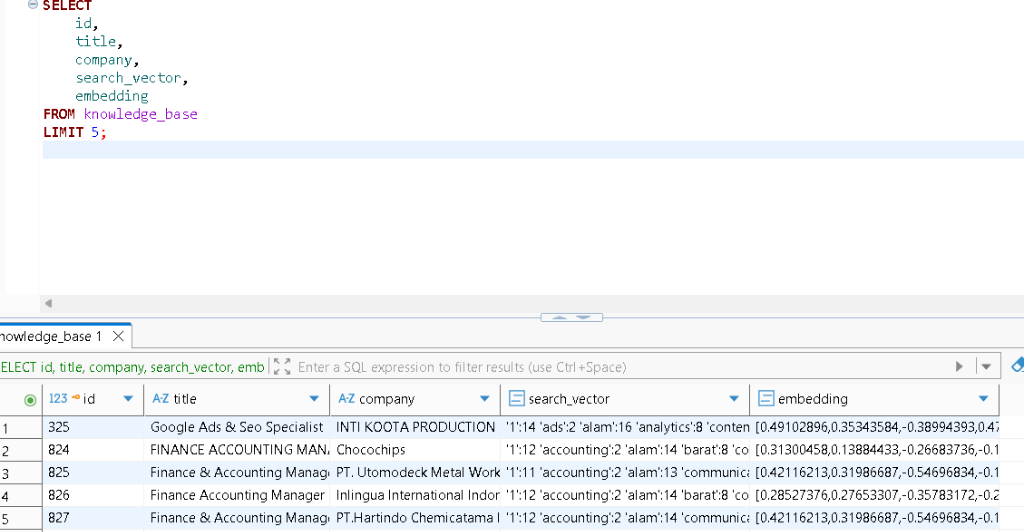
\includegraphics[width=\textwidth]{figures/gambar_4_7_db_embedding.png}
  \caption{Tangkapan Layar Data Vektor dan Leksikal pada PostgreSQL (DBeaver)}
  \label{fig:db_embedding}
\end{figure}

\subsubsection{Verifikasi dan Analisis Dataset Akhir}

\textbf{1. Verifikasi Data (Bukti Eksistensi)}

Untuk memvalidasi keberadaan data secara empiris setelah tahapan ekstraksi dan pembersihan (ETL), query SQL dasar dilakukan langsung pada basis data PostgreSQL. Gambar \ref{fig:sql_count} membuktikan bahwa sistem telah sukses menyimpan total 720 dokumen dengan kalkulasi entri yang \textit{non-null}. Gambar \ref{fig:sql_cluster} mengonfirmasi bahwa distribusi per klaster persis mencapai angka 90 dokumen per klaster tanpa adanya anomali.

\begin{figure}[H]
  \centering
  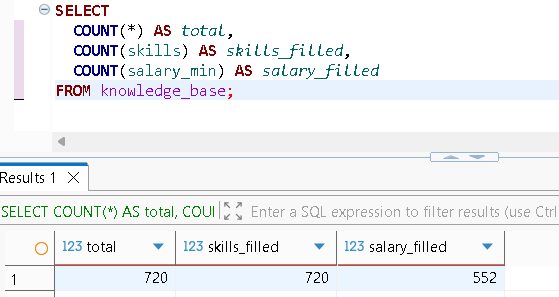
\includegraphics[width=0.8\textwidth]{figures/screenshot_sql_count.png}
  \caption{Hasil Eksekusi Query Agregasi Total Data dan Kelengkapan Kolom}
  \label{fig:sql_count}
\end{figure}

\begin{figure}[H]
  \centering
  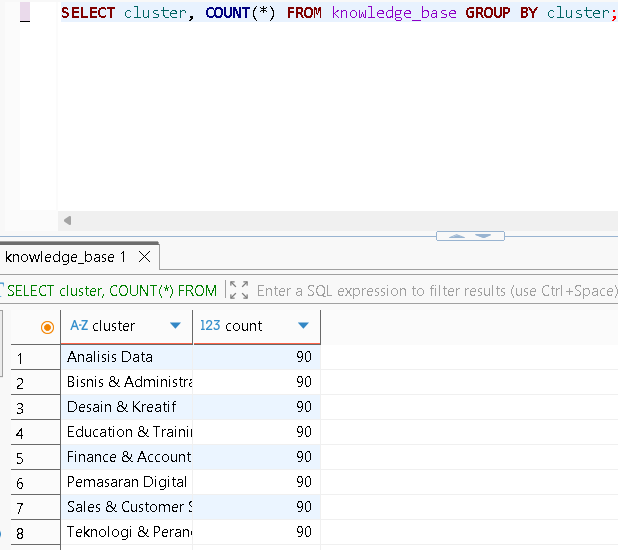
\includegraphics[width=0.8\textwidth]{figures/screenshot_sql_cluster.png}
  \caption{Hasil Eksekusi Query Distribusi Data per Klaster Karier}
  \label{fig:sql_cluster}
\end{figure}

\textbf{2. Karakteristik Dataset (\textit{Data Completeness})}

Sebagian besar data diekstrak dengan tingkat kelengkapan yang sempurna karena mekanisme \textit{scraper} dirancang untuk membuang elemen DOM yang rusak. Namun, platform sumber (Glints) menetapkan transparansi gaji (\textit{salary}) sebagai kolom opsional bagi perusahaan. Tabel \ref{tab:deskriptif_kolom} meringkas status kelengkapan data hasil ekstraksi tersebut.

\begin{table}[H]
\centering
\caption{Ringkasan Karakteristik Kolom \textit{Knowledge Base}}
\label{tab:deskriptif_kolom}
\begin{tabular}{lccl}
\toprule
\textbf{Kolom} & \textbf{Total Terisi} & \textbf{NULL} & \textbf{Keterangan} \\
\midrule
\texttt{title} & 720 & 0 & Wajib ada pada elemen DOM \\
\texttt{company} & 720 & 0 & Wajib ada pada elemen DOM \\
\texttt{location} & 720 & 0 & Wajib ada pada elemen DOM \\
\texttt{skills} & 720 & 0 & Wajib terisi minimal 1 entitas \\
\texttt{salary\_text} & 552 & 168 & Teks gaji asli dari scraping \\
\texttt{salary\_min} & 552 & 168 & Hasil parsing ke Rupiah (integer) \\
\texttt{salary\_max} & 552 & 168 & Hasil parsing ke Rupiah (integer) \\
\bottomrule
\end{tabular}
\end{table}

\textbf{3. Visualisasi Analisis Data (\textit{Exploratory Data Analysis})}

Visualisasi menggunakan pustaka \textit{Matplotlib} pada Python (Gambar \ref{fig:distribusi_dataset}) disusun untuk memperjelas karakteristik dataset. Grafik batang secara gamblang mendemonstrasikan pemerataan klaster tanpa adanya \textit{skewness} pada kategori tertentu. Di sisi lain, \textit{pie chart} menggarisbawahi bahwa mayoritas lowongan (76,7\%) secara transparan menyertakan rentang gaji (552 dari 720 data), yang mana keberadaan data ini akan secara signifikan memperkaya dimensi rekomendasi NusaNara ketika pengguna mengemukakan preferensi kompensasi finansial yang spesifik.

\begin{figure}[H]
  \centering
  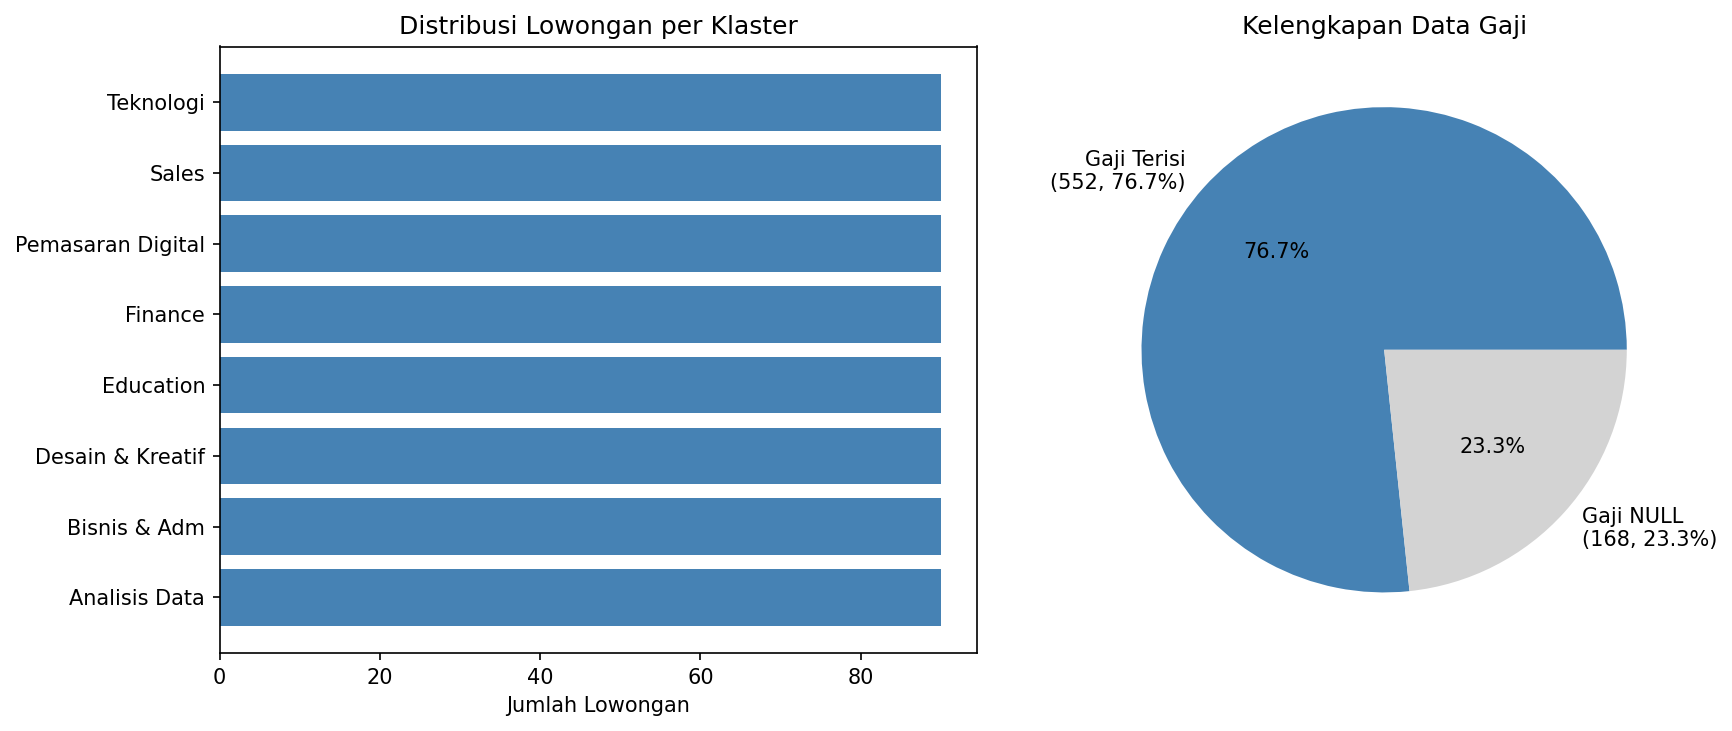
\includegraphics[width=\textwidth]{figures/distribusi_dataset.png}
  \caption{Analisis Distribusi Lowongan dan Kelengkapan Data Gaji}
  \label{fig:distribusi_dataset}
\end{figure}
\subsubsection{Skema Basis Data}
Setiap lowongan disimpan dalam tabel \texttt{knowledge\_base} dengan skema berikut:

\begin{table}[H]
\centering
\caption{Skema Tabel \texttt{knowledge\_base} pada PostgreSQL 16}
\label{tab:schema}
\begin{tabularx}{\textwidth}{llX}
\toprule
\textbf{Kolom} & \textbf{Tipe Data} & \textbf{Keterangan} \\
\midrule
\texttt{id} & SERIAL & Primary key auto-increment \\
\texttt{title} & TEXT & Judul posisi pekerjaan \\
\texttt{company} & TEXT & Nama perusahaan \\
\texttt{location} & TEXT & Kota/provinsi \\
\texttt{salary\_text} & TEXT & Teks gaji asli dari scraping (opsional) \\
\texttt{salary\_min} & INTEGER & Gaji minimum dalam Rupiah (hasil parsing) \\
\texttt{salary\_max} & INTEGER & Gaji maksimum dalam Rupiah (hasil parsing) \\
\texttt{skills} & TEXT[] & Array keterampilan \\
\texttt{cluster} & TEXT & Salah satu dari 8 klaster karier \\
\texttt{content} & TEXT & Narasi gabungan untuk embedding \\
\texttt{embedding} & VECTOR(768) & Representasi vektor nomic-embed \\
\texttt{search\_vector} & TSVECTOR & Indeks full-text search \\
\bottomrule
\end{tabularx}
\end{table}

Kolom \texttt{embedding} diisi oleh pipeline Task 04 menggunakan model
\texttt{nomic-embed-text-v2-moe} (768 dimensi), diindeks dengan algoritma IVFFlat
untuk mempercepat pencarian ANN. Kolom \texttt{search\_vector} dibangkitkan otomatis
menggunakan fungsi \texttt{to\_tsvector('simple', ...)}.

\subsubsection{Analisis Ruang Vektor: Visualisasi Distribusi Semantik 8 Klaster}

Guna memverifikasi secara empiris bahwa model \textit{embedding} yang digunakan (\texttt{nomic-embed-text-v2-moe}) mampu membedakan profesi secara semantik, seluruh 720 vektor berdimensi 768 yang tersimpan di dalam basis data PostgreSQL dianalisis secara komputasional. Karena ruang 768 dimensi tidak dapat divisualisasikan secara langsung, dilakukan reduksi dimensi dua tahap: (1) \textit{Principal Component Analysis} (PCA) mereduksi dari 768 ke 50 dimensi (mempertahankan 72,7\% varian total), kemudian (2) algoritma \textit{t-Distributed Stochastic Neighbor Embedding} (t-SNE) \cite{VanDerMaaten2008} memproyeksikan representasi 50D tersebut ke dalam ruang 2D yang dapat divisualisasikan, dengan parameter \textit{perplexity} = 40 dan 1.000 iterasi optimasi.

\begin{figure}[H]
  \centering
  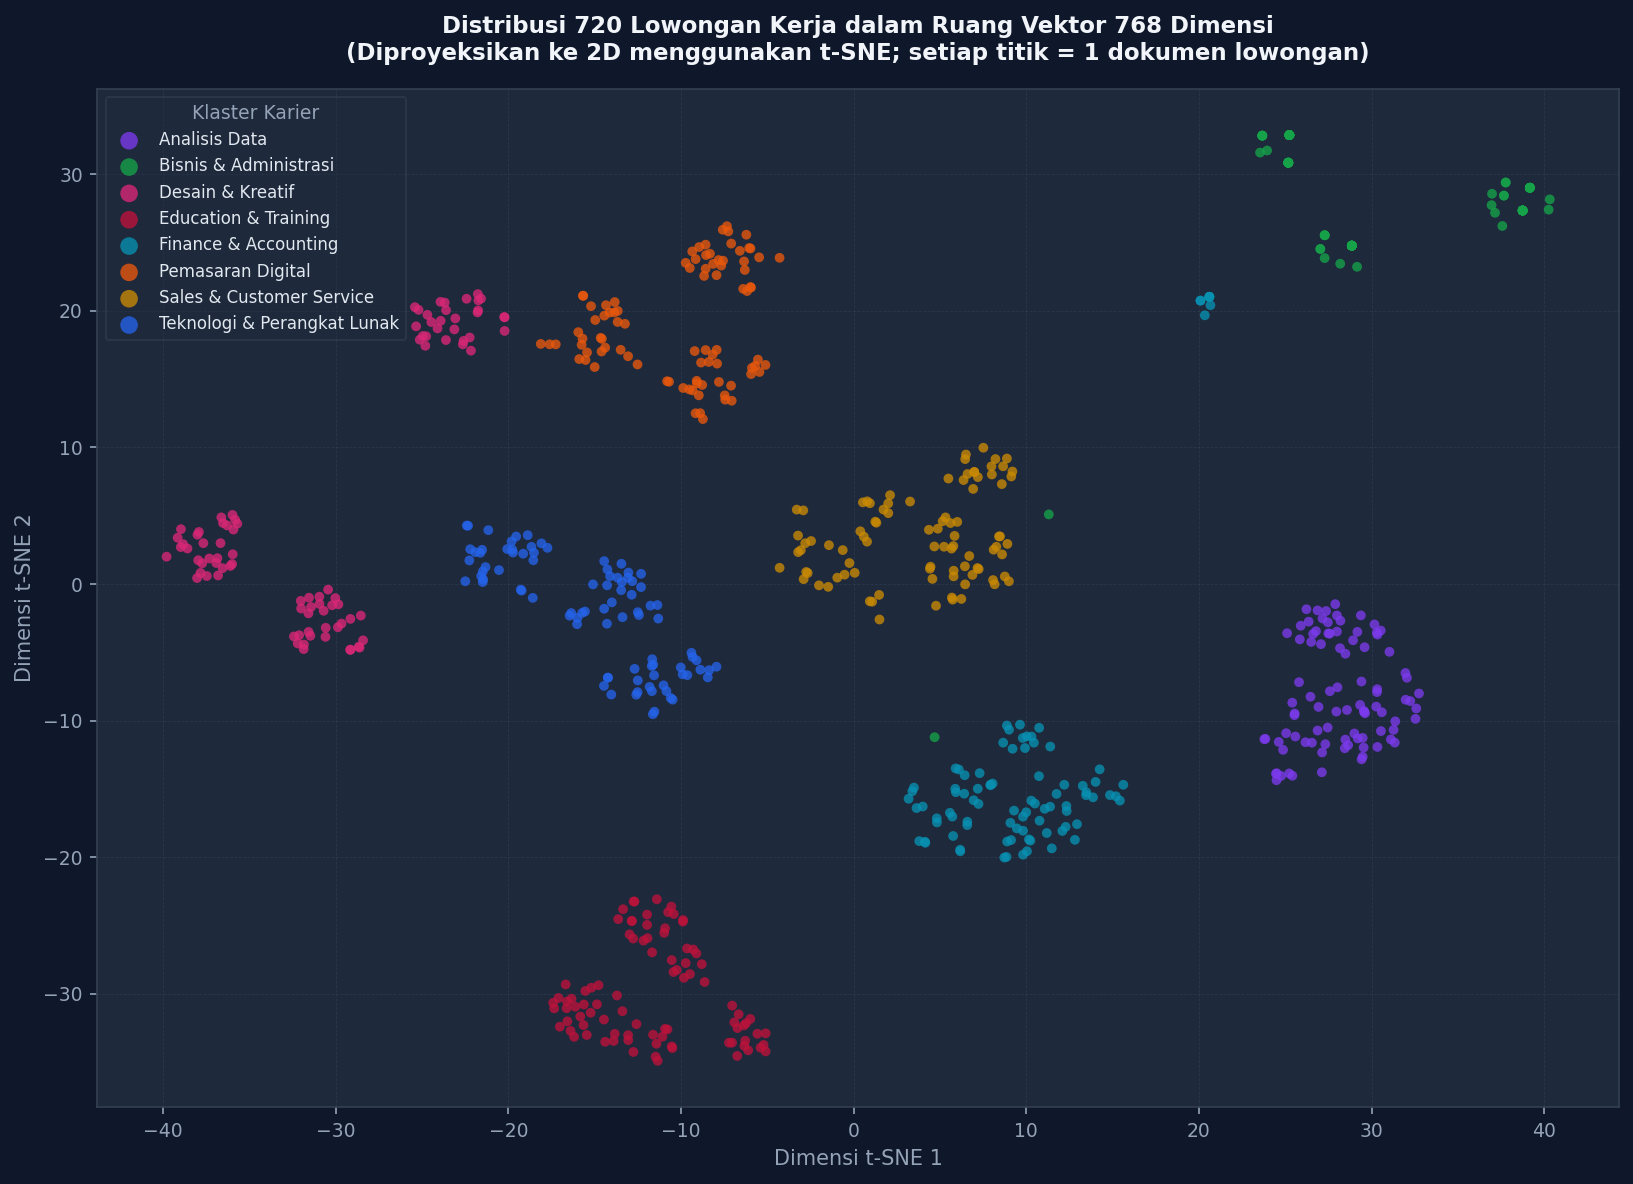
\includegraphics[width=\textwidth]{figures/gambar_4_8_tsne_cluster.png}
  \caption{Visualisasi t-SNE Distribusi 720 Lowongan dalam Ruang Vektor 768 Dimensi (setiap titik merepresentasikan satu dokumen lowongan, diwarnai sesuai klaster kariernya)}
  \label{fig:tsne_cluster}
\end{figure}

Hasil proyeksi t-SNE pada Gambar \ref{fig:tsne_cluster} memberikan bukti visual yang sangat kuat. Titik-titik dari klaster yang sama secara konsisten membentuk gugus (\textit{cluster}) yang kompak dan terpisah satu sama lain dalam ruang 2D, meskipun tidak ada informasi label klaster yang digunakan selama proses \textit{embedding} --- model hanya menerima teks mentah. Fenomena ini membuktikan bahwa \texttt{nomic-embed-text-v2-moe} berhasil mengkodekan \textit{semantic proximity} yang bermakna secara domain: lowongan ``Data Analyst'' dan ``Data Scientist'' berada pada gugus yang berdekatan (Analisis Data), sementara terdapat pemisahan yang jelas antara klaster ``Education \& Training'' dengan ``Finance \& Accounting''. Keterpisahan yang konsisten ini merupakan prasyarat fundamental agar komponen \textit{semantic search} dalam \textit{Hybrid Search} dapat bekerja dengan akurasi tinggi.

\subsubsection{Visualisasi Mekanisme Retrieval RAG dalam Ruang Vektor}

Untuk mendemonstrasikan bagaimana sistem RAG mengeksekusi pencarian dalam konteks nyata, dilakukan simulasi satu kueri pengguna (\textit{``Saya mahasiswa Sistem Informasi, mahir Python dan SQL, tertarik di bidang Data Analyst''}) secara \textit{end-to-end}. Narasi tersebut diubah menjadi vektor 768 dimensi menggunakan model \textit{embedding} yang identik. Dalam implementasi produksi, pencarian dilakukan oleh \textbf{pgvector} menggunakan operator \textit{Cosine Distance} (\texttt{<=>}) dengan akselerasi indeks \textit{IVFFlat} --- sebuah algoritma \textit{Approximate Nearest Neighbor} (ANN) yang lebih efisien secara komputasi dibandingkan \textit{exact} KNN untuk skala dokumen besar. Skor \textit{Cosine Similarity} (dikonversi dari jarak: $sim = 1 - dist$) kemudian digunakan untuk menentukan Top-K kandidat semantik.

\begin{figure}[H]
  \centering
  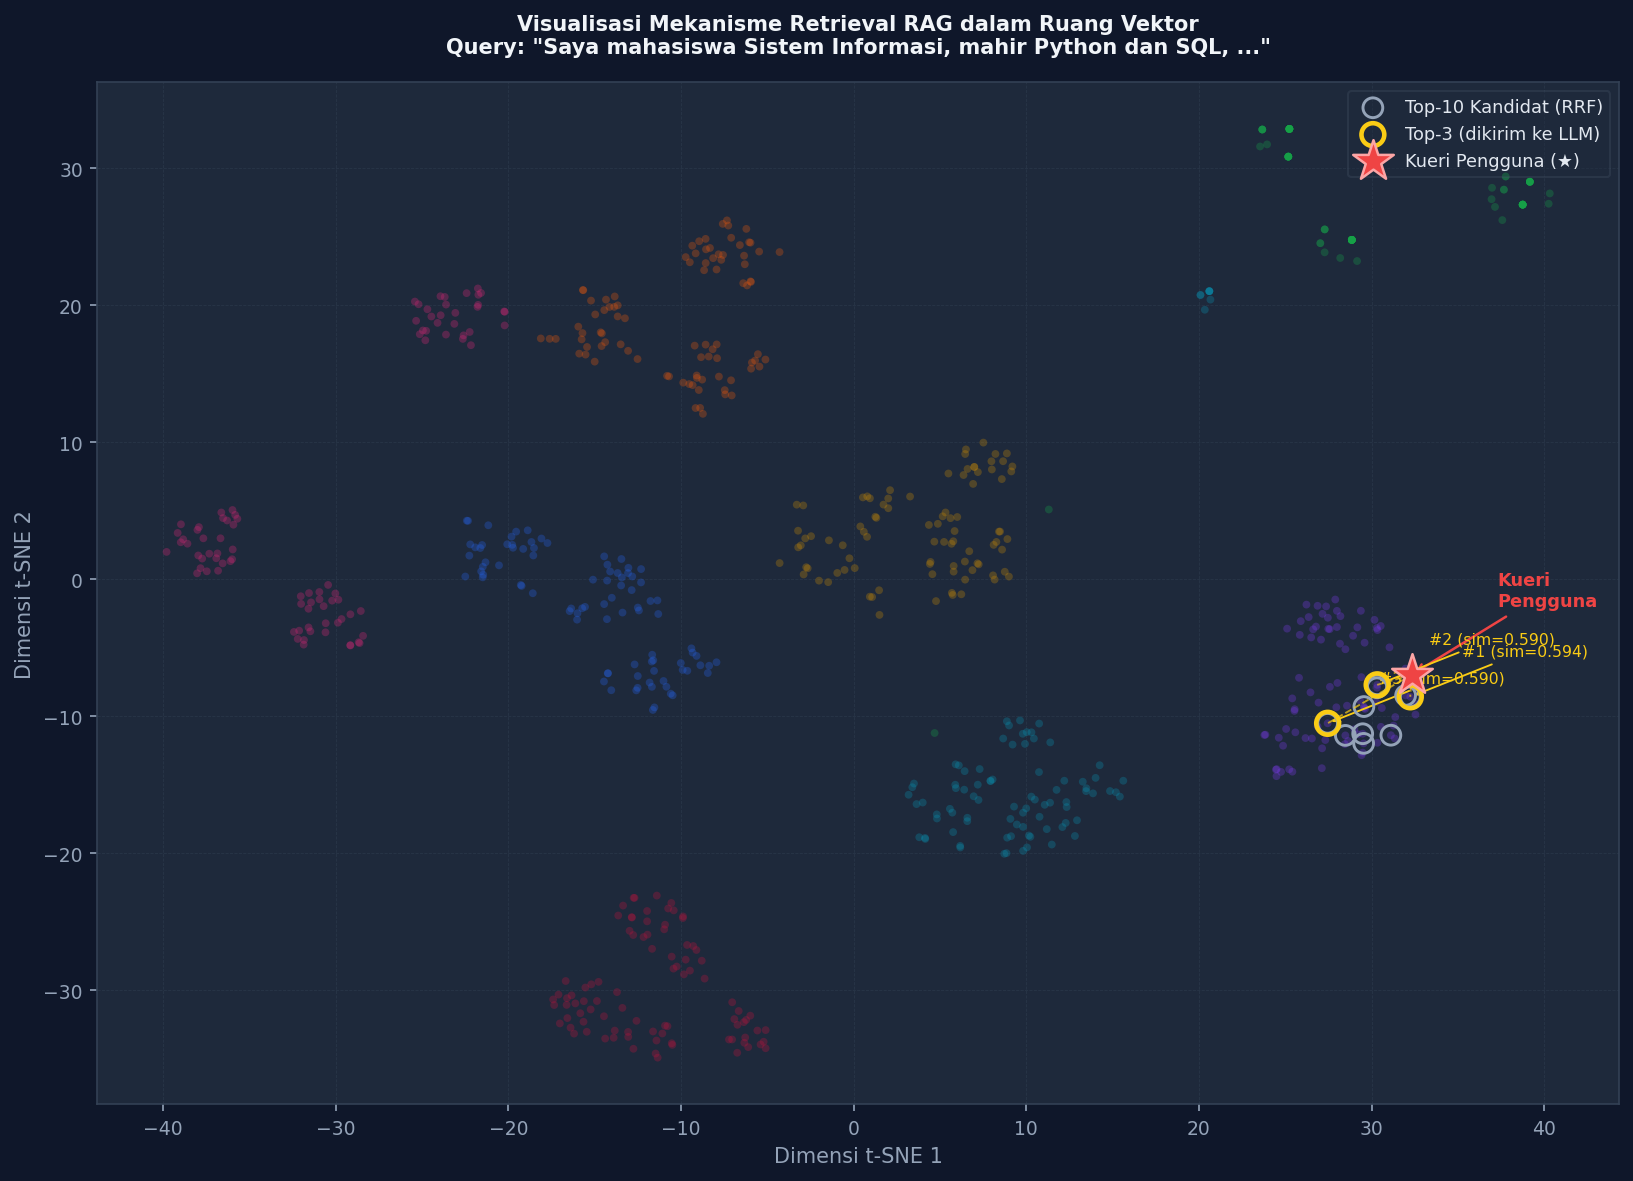
\includegraphics[width=\textwidth]{figures/gambar_4_9_retrieval_knn.png}
  \caption{Visualisasi Mekanisme \textit{Semantic Search} (ANN via IVFFlat/pgvector): Posisi Kueri Pengguna (bintang merah $\star$) dan Dokumen Terambil (Top-10 lingkaran abu-abu; Top-3 lingkaran emas) dalam Proyeksi t-SNE}
  \label{fig:retrieval_knn}
\end{figure}

Gambar \ref{fig:retrieval_knn} mengilustrasikan mekanisme \textit{Approximate Nearest Neighbor} (ANN) yang mendasari komponen \textit{vector search} dalam \textit{Hybrid Search}. Bintang merah ($\star$) merepresentasikan posisi kueri pengguna setelah diproyeksikan ke ruang 2D, sementara dokumen-dokumen yang terambil sebagai Top-10 (ditandai lingkaran abu-abu) dan Top-3 (ditandai lingkaran emas dengan garis penghubung) terlihat jelas berposisi di \textbf{dalam klaster Analisis Data} --- yang secara semantik paling dekat dengan narasi karier pengguna. Sebagaimana tampak pada label anotasi dalam gambar, tiga dokumen teratas yang akhirnya dikirimkan ke LLM sebagai konteks memiliki skor \textit{Cosine Similarity} berturut-turut: \textbf{\#1 (sim = 0,594)}, \textbf{\#2 (sim = 0,590)}, dan \textbf{\#3 (sim = 0,590)} --- semuanya merupakan posisi Data Analyst dari perusahaan-perusahaan berbeda, yang secara intuitif sesuai dengan profil yang dideskripsikan dalam narasi. Perlu dicatat bahwa visualisasi ini menggunakan \textit{exact} Cosine Similarity untuk keperluan ilustrasi yang lebih jelas, sementara implementasi produksi menggunakan ANN (IVFFlat) yang hasilnya secara empiris ekuivalen pada skala 720 dokumen.

\subsubsection{Analisis Kohesi Semantik Intra-Klaster (Cosine Similarity)}

Evaluasi kuantitatif kualitas representasi vektor dilanjutkan dengan mengukur \textit{Cosine Similarity} antar-dokumen dalam masing-masing klaster (\textit{intra-cluster similarity}). Metrik ini mengukur seberapa erat seluruh 90 dokumen dalam satu klaster saling berkaitan secara semantik; nilai yang tinggi mengindikasikan model berhasil memetakan dokumen-dokumen satu bidang ke zona yang kompak dalam ruang vektor.

\begin{figure}[H]
  \centering
  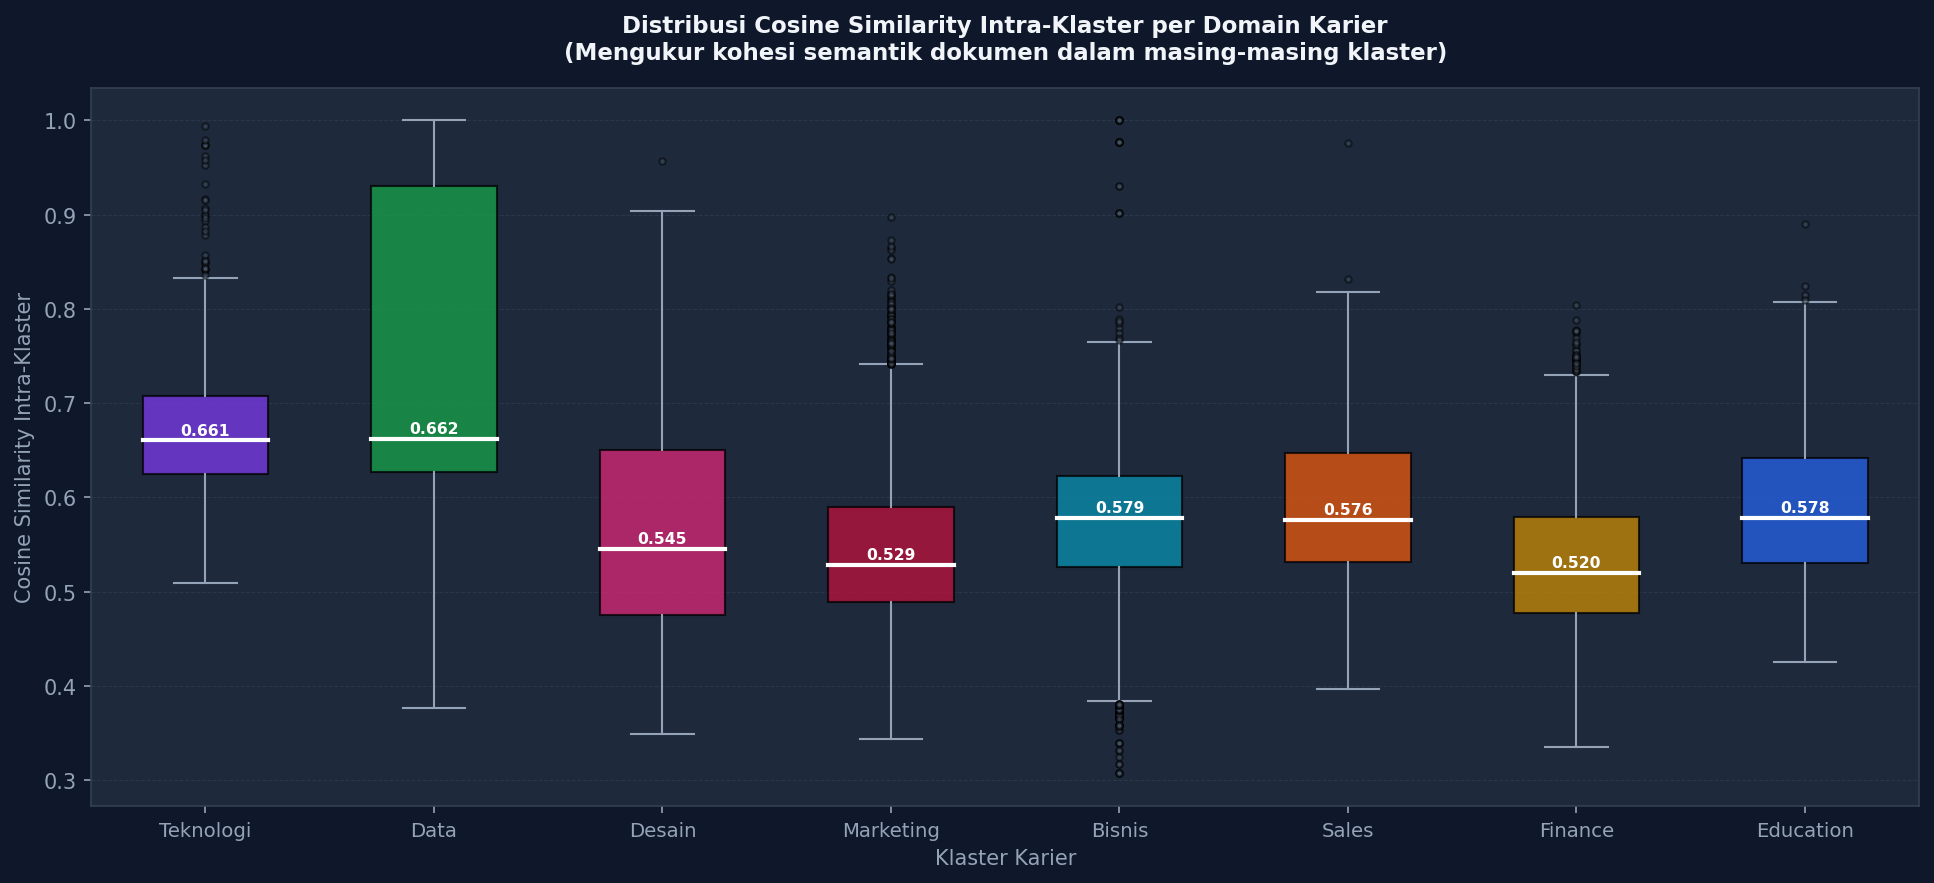
\includegraphics[width=\textwidth]{figures/gambar_4_10_cosine_boxplot.png}
  \caption{Distribusi \textit{Cosine Similarity} Intra-Klaster per Domain Karier (Boxplot; garis putih = nilai median)}
  \label{fig:cosine_boxplot}
\end{figure}

Gambar \ref{fig:cosine_boxplot} menyajikan distribusi \textit{intra-cluster similarity} ke-8 klaster. Beberapa temuan kunci dapat diidentifikasi:

\begin{itemize}[noitemsep]
  \item \textbf{Kohesi Tertinggi:} Klaster \textit{Analisis Data} (median = 0,662) dan \textit{Teknologi \& Perangkat Lunak} (median = 0,661) memiliki kohesi semantik tertinggi. Kedua klaster ini mencakup lowongan dengan terminologi teknis yang sangat spesifik dan konsisten (misal: \textit{Python, SQL, Machine Learning, React, DevOps}), sehingga dokumen-dokumen di dalamnya menghasilkan representasi vektor yang sangat homogen.
  \item \textbf{Kohesi Terendah:} Klaster \textit{Finance \& Accounting} (median = 0,520) dan \textit{Pemasaran Digital} (median = 0,529) menunjukkan variabilitas lebih tinggi. Hal ini dapat dijelaskan oleh keragaman sub-domain yang luas: klaster Finance mencakup posisi mulai dari \textit{Tax Consultant} hingga \textit{Financial Analyst}, sementara Pemasaran Digital mencakup \textit{SEO Specialist}, \textit{Content Creator}, hingga \textit{Google Ads Specialist} --- masing-masing dengan vokabuler yang berbeda meski berada dalam satu klaster.
  \item \textbf{Grand Median Keseluruhan:} Nilai 0,577 (rata-rata dari seluruh median klaster) secara konsisten berada di atas ambang batas kemiripan semantik yang bermakna (0,5), membuktikan bahwa seluruh \textit{Knowledge Base} tersusun dengan baik secara representasi vektor dan tidak mengandung \textit{noise} dokumentasi yang signifikan.
\end{itemize}

Ketiga analisis di atas --- distribusi t-SNE, mekanisme \textit{Semantic Search} (ANN/IVFFlat), dan distribusi \textit{Cosine Similarity} --- secara kolektif membuktikan bahwa fondasi \textit{Knowledge Base} NusaNara memiliki kualitas representasi semantik yang tinggi dan layak digunakan sebagai basis bagi sistem RAG produksi.



% -------------------------------------------------------
\subsection{Implementasi Sistem}
% -------------------------------------------------------

\subsubsection{Spesifikasi Lingkungan Produksi (VPS)}

Sistem NusaNara di-\textit{deploy} pada VPS \textit{dedicated} dengan lokasi
\textit{data center} di Jakarta, Indonesia. Pemilihan lokasi ini bertujuan
meminimalkan latensi jaringan bagi pengguna target.

\begin{table}[H]
\centering
\caption{Spesifikasi Perangkat Keras VPS Produksi}
\label{tab:spesifikasi_hw}
\begin{tabular}{ll}
\toprule
\textbf{Komponen} & \textbf{Spesifikasi} \\
\midrule
CPU & 4 vCPU \\
RAM & 16 GB \\
Storage & 100 GB SSD (RAID 10) \\
Jaringan & Dedicated IPv4, Unlimited Bandwidth \\
Data Center & Jakarta, Indonesia \\
Sistem Operasi & Ubuntu 22.04 LTS \\
\bottomrule
\end{tabular}
\end{table}

Pemilihan 4 vCPU dan 16 GB RAM merupakan keputusan teknis yang dipertimbangkan
berdasarkan kebutuhan eksekusi \textit{Large Language Model} (LLM) secara lokal.
Model Llama 3 dipilih dalam varian \textbf{8B parameter (4-bit Quantized)}
(bukan versi 70B) agar dapat beroperasi pada RAM 16 GB. Walaupun sistem menggunakan
dua agen LLM (\textit{Main RAG Agent} dan \textit{Extractor Agent}), Ollama mengelola
memori dengan memuat bobot model hanya satu kali. Kedua agen tersebut mengakses
model secara bergantian (berbagi \textit{instance} memori yang sama), sehingga
\textit{bottleneck} memori dapat dihindari.

\begin{table}[H]
\centering
\caption{Spesifikasi Perangkat Lunak Produksi}
\label{tab:spesifikasi_sw}
\begin{tabularx}{\textwidth}{llX}
\toprule
\textbf{Komponen} & \textbf{Teknologi} & \textbf{Versi/Detail} \\
\midrule
Web Server & Nginx & Reverse Proxy, SSL Termination \\
Process Manager & Systemd & \texttt{nusanara.service}, \texttt{Restart=always} \\
SSL/TLS & Let's Encrypt & Auto-renew via Certbot \\
Firewall & UFW & Port 5432, 11434, 8000 -- internal only \\
\midrule
Runtime Backend & Python & 3.11 \\
Web Framework & FastAPI + Uvicorn & ASGI \\
Database & PostgreSQL & 16 + pgvector (VECTOR(768), IVFFlat) \\
DB Driver & asyncpg & Async, connection pooling \\
LLM Platform & Ollama & Local inference \\
LLM (Generator \& Extractor) & Llama 3.1 & \textbf{8B parameter (4-bit Quantized)} \\
Embedding Model & nomic-embed-text-v2-moe & 768 dimensi, MoE \\
\midrule
Frontend & Next.js & 14 (App Router, TypeScript) \\
Auth Provider & Clerk & JWT RS256 \\
Frontend Hosting & Vercel & CDN Global \\
\bottomrule
\end{tabularx}
\end{table}

\subsubsection{Implementasi Pipeline RAG}

Pipeline RAG diimplementasikan dalam \texttt{backend/services/llm\_service.py}.
Alur eksekusi untuk setiap permintaan rekomendasi:

\begin{lstlisting}[language=Python, caption={Alur pipeline RAG di \texttt{llm\_service.py}}]
async def generate_recommendation(narrative, user_id, pool):
    # 1. Query Expansion
    expanded = await _expand_query(narrative)

    # 2. Embedding (nomic-embed-text-v2-moe)
    vector = await get_embedding(f"search_query: {expanded}")

    # 3. Hybrid Search via RRF
    candidates = await hybrid_search(vector, expanded, top_k=10)

    # 4. Re-ranking heuristik
    top3 = rerank(candidates, user_profile.skills, top_n=3)

    # 5. Build prompt Decision Intelligence
    prompt = build_prompt(narrative, top3, user_profile)

    # 6. LLM Stream (Llama 3.1, stream=True)
    async for token in ollama_stream(prompt):
        yield f"data: {token}\n\n"

    # 7. Simpan history
    await save_history(user_id, narrative, top3, full_response)

    # 8. Background task (NON-BLOCKING)
    asyncio.create_task(
        extract_and_update_profile(user_id, narrative, pool)
    )
    yield "data: [DONE]\n\n"
\end{lstlisting}

\textbf{Fungsi Hybrid Search dengan RRF:}

Implementasi \textit{Hybrid Search} menggabungkan dua paradigma pencarian yang saling
melengkapi. Pencarian semantik menangkap kesamaan makna (misalnya ``programmer'' cocok
dengan ``software engineer'' meskipun kata-katanya berbeda), sedangkan pencarian leksikal
menangkap kecocokan kata kunci eksak (misalnya nama teknologi ``PostgreSQL'' yang harus
muncul literal dalam dokumen).

\begin{lstlisting}[language=Python, caption={Implementasi Hybrid Search dan RRF}]
async def hybrid_search(query_vector, query_text, top_k=10):
    # Set probes untuk optimasi IVFFlat
    await pool.execute("SET LOCAL ivfflat.probes = 3;")

    # Pencarian Semantik (pgvector cosine similarity)
    semantic = await pool.fetch("""
        SELECT id, title, content, skills, cluster,
               1 - (embedding <=> $1) AS cosine_sim,
               ROW_NUMBER() OVER (ORDER BY embedding <=> $1) AS rank
        FROM knowledge_base LIMIT 20
    """, query_vector)

    # Pencarian Full-Text (tsvector)
    lexical = await pool.fetch("""
        SELECT id,
               ROW_NUMBER() OVER (ORDER BY ts_rank DESC) AS rank
        FROM (SELECT id, ts_rank(search_vector, q) AS ts_rank
              FROM knowledge_base, plainto_tsquery('simple',$1) q
              WHERE search_vector @@ q LIMIT 20) sub
    """, query_text)

    # RRF Fusion: skor = 1/(60+rank_sem) + 1/(60+rank_lex)
    rrf = {}
    for doc in semantic:
        rrf[doc['id']] = 1.0 / (60 + doc['rank'])
    for doc in lexical:
        rrf[doc['id']] = rrf.get(doc['id'], 0) + 1.0/(60+doc['rank'])

    return sorted(rrf.items(), key=lambda x: x[1], reverse=True)[:top_k]
\end{lstlisting}

\noindent \textbf{Penjelasan kode baris per baris:}
\begin{itemize}
  \item \textbf{Baris 4--7 (Pencarian Semantik):} Operator \texttt{<=>} adalah operator
    \textit{cosine distance} bawaan pgvector. Ekspresi \texttt{1 - (embedding <=> \$1)}
    mengonversi distance menjadi similarity. \texttt{ROW\_NUMBER()} memberikan peringkat
    1, 2, 3, ... berdasarkan kemiripan. \texttt{LIMIT 20} mengambil 20 teratas.
  \item \textbf{Baris 10--15 (Pencarian Leksikal):} Operator \texttt{@@} mencocokkan
    \texttt{tsvector} dengan \texttt{tsquery}. Fungsi \texttt{ts\_rank()} menghitung
    skor relevansi leksikal berdasarkan frekuensi kemunculan kata kunci.
    \texttt{plainto\_tsquery('simple', ...)} menggunakan konfigurasi 'simple' (tanpa stemming)
    karena nama teknologi dan posisi tidak boleh di-stem.
  \item \textbf{Baris 18--22 (RRF Fusion):} Setiap dokumen mendapat skor
    $\frac{1}{60 + rank}$ dari masing-masing pencarian. Dokumen yang muncul di kedua
    pencarian mendapat akumulasi skor yang lebih tinggi. Konstanta $k=60$ memastikan
    perbedaan peringkat yang berdekatan tidak terlalu drastis.
\end{itemize}

\textbf{Fungsi Re-ranking Heuristik:}

Setelah RRF menghasilkan Top-10 kandidat, sistem menerapkan formula \textit{re-ranking}
heuristik (Persamaan~\ref{eq:rerank} pada Bab~3) dengan tiga dokumen skor tertinggi
dikirim sebagai konteks ke LLM.

\subsubsection{Prompt Decision Intelligence}
\label{subsec:prompt_di}

Prompt LLM dirancang sebagai \textit{Explainable AI} yang mengharuskan model hanya
menggunakan dokumen dari Top-3 retrieval (\textit{faithfulness constraint}) dan
menyertakan skor kuantitatif secara eksplisit. Desain prompt mengikuti prinsip
\textit{structured output} --- di mana LLM diberikan template yang ketat untuk
memastikan konsistensi format output di seluruh sesi.

\begin{table}[H]
\centering
\caption{Struktur 5 Seksi Output Wajib Prompt Decision Intelligence}
\label{tab:prompt}
\begin{tabularx}{\textwidth}{clX}
\toprule
\textbf{Seksi} & \textbf{Judul} & \textbf{Konten Wajib} \\
\midrule
1 & Analisis Profil \& Trade-off & Strengths, weaknesses, trade-off karier \\
2 & Rekomendasi Keputusan & Top-3 posisi + \textbf{Skor RAG} + \textbf{Overlap Skill} + Action Plan 7 Hari \\
3 & Analisis Skill Gap & Gap konkret antara profil dan persyaratan \\
4 & Rencana Pengembangan Skill & Roadmap skill spesifik \\
5 & Insight Pasar Kerja Lokal & Tren, gaji, dan peluang di Indonesia \\
\bottomrule
\end{tabularx}
\end{table}

\textbf{Penjelasan mekanisme faithfulness constraint:}
\begin{itemize}
  \item Prompt secara eksplisit menyertakan instruksi:
    ``\textit{HANYA gunakan informasi dari dokumen yang disediakan. JANGAN mengarang
    posisi, perusahaan, atau data yang tidak ada dalam konteks.}''
  \item Setiap rekomendasi posisi wajib menyertakan \textbf{Skor RAG} (cosine similarity
    antara query dan dokumen, diambil dari tahap retrieval) dan \textbf{Overlap Skill}
    (jumlah skill pengguna yang cocok dengan persyaratan dokumen, diambil dari
    tahap re-ranking). Kedua metrik ini bersifat \textit{traceable} --- pengguna dan
    peneliti dapat memverifikasi apakah LLM benar-benar menggunakan dokumen yang
    disediakan atau berhalusinasi.
  \item Template diinjeksikan ke \texttt{system prompt} dengan format:
    ``Kamu adalah NusaNara AI Career Advisor. Berikut profil pengguna: [profil].
    Berikut narasi pengguna: [narasi]. Berikut Top-3 rekomendasi dari database:
    [dokumen 1], [dokumen 2], [dokumen 3]. Berikan analisis dalam 5 seksi berikut...''
\end{itemize}

\textbf{Konfigurasi LLM untuk generasi:}
\begin{itemize}[noitemsep]
  \item \texttt{temperature = 0.7}: Cukup kreatif untuk narasi yang bervariasi,
    namun cukup deterministik untuk konsistensi rekomendasi.
  \item \texttt{num\_predict = 2048}: Batas token output yang cukup untuk 5 seksi
    terstruktur ($\sim$500--800 kata).
  \item \texttt{stream = True}: Mengaktifkan SSE streaming untuk TTFB optimal.
\end{itemize}

\subsubsection{Adaptive Profile System}

Modul \texttt{memory\_service.py} mengimplementasikan sistem personalisasi menggunakan
arsitektur \textbf{hybrid dua tahap}: (1) LLM \textit{Extractor Agent} untuk mengubah
narasi tidak terstruktur menjadi data terstruktur, dan (2) logika \textit{rule-based}
deterministik untuk memperbarui database.

\paragraph{Tahap 1 -- LLM Extractor Agent}
Input pengguna berupa narasi teks bebas (bahasa campur Indonesia-Inggris, gaya informal)
tidak mungkin diproses menggunakan \textit{rule-based} murni (regex, NER sederhana) karena
variasi linguistik yang tinggi. Oleh karena itu, Llama 3.1 8B (4-bit) digunakan sebagai
\textit{Extractor Agent} dengan \texttt{temperature=0.1} (hampir deterministik) dan
\texttt{num\_predict=200} (output pendek, hanya JSON).

\begin{lstlisting}[language=Python, caption={Prompt dan pemanggilan LLM Extractor Agent}]
_EXTRACTOR_PROMPT = """Kamu adalah extractor data profil.
Dari narasi pengguna di bawah, ekstrak informasi
dalam format JSON STRICT.

NARASI: {narrative}

INSTRUKSI:
1. Ekstrak semua skill teknis yang DISEBUTKAN
2. Ekstrak minat karier yang jelas
3. Buat ringkasan profil 1-2 kalimat (Bahasa Indonesia)
4. Jika narasi tidak mengandung info relevan, kembalikan []

WAJIB kembalikan JSON (TANPA teks lain):
{{"skills": [], "interests": [], "summary_update": "..."}}"""

async def _call_extractor(narrative: str) -> dict | None:
    resp = await client.post(
        f"{OLLAMA_URL}/api/generate",
        json={"model": "llama3.1",  # 8B parameter (4-bit Quantized)
              "prompt": prompt,
              "stream": False,
              "options": {"temperature": 0.1, "num_predict": 200}}
    )
    raw = resp.json()["response"].strip()
    return json.loads(raw[raw.find("{"):raw.rfind("}")+1])
\end{lstlisting}

Contoh transformasi:
\begin{quote}
\small
\textbf{Input narasi:} ``Saya mahasiswa informatika, lumayan jago Python sama SQL,
pengen kerja di bidang data science''\\
\textbf{Output JSON:} \texttt{\{"skills":["Python","SQL"], "interests":["data science"],
"summary\_update":"Mahasiswa informatika dengan keahlian Python dan SQL..."\}}
\end{quote}

\paragraph{Tahap 2 -- Deterministic Merge (Rule-Based)}
Setelah LLM menghasilkan JSON terstruktur, update database dilakukan
sepenuhnya secara \textit{rule-based} tanpa LLM:

\begin{lstlisting}[language=Python, caption={Logika UNION merge deterministik}]
async def _update_profile(conn, user_id, new_skills, new_interests, summary):
    current = await conn.fetchrow(
        "SELECT identified_skills, career_interests "
        "FROM user_profiles WHERE user_id=$1", user_id
    )
    # UNION set -- skill lama TIDAK PERNAH hilang
    merged_skills = list(set(current["identified_skills"] or [])
                         | set(new_skills))
    merged_interests = list(set(current["career_interests"] or [])
                            | set(new_interests))

    await conn.execute("""
        UPDATE user_profiles
        SET identified_skills=$2, career_interests=$3,
            profile_summary=$4, session_count=session_count+1,
            last_active=NOW()
        WHERE user_id=$1
    """, user_id, merged_skills, merged_interests, summary)
\end{lstlisting}

Properti desain \textit{Adaptive Profile System}:
\begin{itemize}
  \item \textbf{Hybrid:} LLM untuk ekstraksi (\textit{unstructured} $\to$ \textit{structured}),
    \textit{rule-based} untuk merge (\textit{structured} $\to$ database).
    Pendekatan ini dipilih setelah mempertimbangkan dua alternatif:
    (a) \textbf{Full-LLM} --- di mana LLM juga melakukan merge. Pendekatan ini
    tidak deterministik; LLM bisa ``lupa'' skill lama, mengubah format, atau
    menghasilkan duplikat yang sulit dideteksi.
    (b) \textbf{Full-rule-based} --- di mana regex atau NER digunakan untuk
    ekstraksi. Pendekatan ini gagal menangani variasi linguistik (code-switching,
    bahasa informal, skill implisit seperti ``bikin UI'' $\Rightarrow$ ``UI/UX Design'').
    Pendekatan hybrid menggabungkan fleksibilitas NLU dari LLM dengan konsistensi
    matematis dari operasi set.
  \item \textbf{Akumulatif \& Idempoten:} Operasi UNION set ($A \cup B$) memastikan
    bahwa skill lama tidak pernah hilang saat skill baru ditambahkan.
    Jika skill ``Python'' sudah ada dan disebutkan lagi, profil tidak berubah ---
    UNION secara definisi mengeliminasi duplikat. Properti ini menjamin bahwa
    urutan sesi tidak memengaruhi hasil akhir (komutatif).
  \item \textbf{Deterministik:} Tidak ada elemen acak (\textit{randomness}) dalam
    proses merge. Untuk input yang sama, output selalu identik.
    Ini berbeda dari tahap LLM yang bersifat \textit{stochastic} ---
    meskipun diminimalisir dengan \texttt{temperature=0.1}.
  \item \textbf{Non-blocking:} Dieksekusi via \texttt{asyncio.create\_task()} setelah
    sinyal \texttt{[DONE]} dikirim ke klien. Proses update profil berjalan sepenuhnya
    di \textit{background}, sehingga tidak menambah latensi pipeline RAG.
    Pengguna sudah menerima rekomendasi lengkap sebelum profil selesai diperbarui.
  \item \textbf{Graceful degradation:} Jika LLM Extractor gagal \textit{parse} JSON
    (misalnya karena timeout atau output malformed), sistem melanjutkan tanpa
    \textit{crash} --- profil tidak diperbarui untuk sesi tersebut, namun
    pipeline RAG tetap berjalan normal. Penanganan error menggunakan
    blok \texttt{try/except} dengan \textit{logging} untuk diagnosis.
\end{itemize}

\subsubsection{Arsitektur Deployment Produksi}

\begin{figure}[H]
  \centering
  
\includegraphics[width=\textwidth]{arsitektur_deployment}
  \caption{Arsitektur Deployment Produksi NusaNara (VPS + Vercel)}
  \label{fig:deployment}
\end{figure}

Sistem dideploy menggunakan arsitektur hybrid sebagaimana pada Gambar \ref{fig:deployment}:
\textit{frontend} di-\textit{host} di Vercel (CDN global), sedangkan \textit{backend},
database, dan LLM dipusatkan di VPS Ubuntu 22.04 (spesifikasi tercantum pada Tabel \ref{tab:spesifikasi_hw}).

\textbf{Justifikasi spesifikasi:}
\begin{itemize}[noitemsep]
  \item \textbf{16 GB RAM:} Alokasi memori: Llama 3.1 8B (4-bit Quantized) ($\sim$5 GB \textit{shared instance}),
    PostgreSQL shared buffers ($\sim$2 GB), nomic-embed ($\sim$1 GB),
    Uvicorn + Python runtime ($\sim$1 GB), OS + buffer ($\sim$7 GB).
  \item \textbf{4 vCPU:} Diperlukan untuk paralelisme inferensi LLM dan
    concurrent database queries dari multiple users.
  \item \textbf{RAID 10 SSD:} Kombinasi striping (kecepatan) dan mirroring
    (redundansi) untuk performa I/O database dan keamanan data.
  \item \textbf{DC Jakarta:} Latensi jaringan minimal ke pengguna Indonesia
    ($<$10ms vs $>$100ms untuk DC Singapura/US).
\end{itemize}

Konfigurasi Nginx kritis untuk SSE:
\begin{lstlisting}[language=bash, caption={Konfigurasi Nginx untuk SSE Streaming}]
location / {
    proxy_pass         http://127.0.0.1:8000;
    proxy_http_version 1.1;
    proxy_buffering    off;    # WAJIB untuk SSE streaming
    proxy_read_timeout 300s;   # Timeout panjang untuk LLM response
}
\end{lstlisting}

\noindent \textbf{Penjelasan konfigurasi:}
\begin{itemize}[noitemsep]
  \item \texttt{proxy\_buffering off}: \textbf{Wajib} untuk SSE. Jika buffering aktif,
    Nginx akan menunggu seluruh respons selesai sebelum mengirim ke klien --- ini
    menghilangkan efek \textit{streaming} dan membuat pengguna menunggu 15--30 detik
    hingga LLM selesai generate. Dengan buffering off, setiap token langsung diteruskan.
  \item \texttt{proxy\_read\_timeout 300s}: LLM mungkin memerlukan waktu lama untuk
    respons panjang. Default Nginx (60 detik) akan memutus koneksi sebelum LLM selesai.
  \item \texttt{proxy\_http\_version 1.1}: Diperlukan agar HTTP \textit{keep-alive}
    berfungsi dengan benar antara Nginx dan Uvicorn.
\end{itemize}

% -------------------------------------------------------
\subsubsection{Sistem Autentikasi: JWT RS256 via Clerk}
\label{subsec:auth_jwt}
% -------------------------------------------------------

Autentikasi sistem NusaNara menggunakan \textbf{JSON Web Token (JWT)} dengan
algoritma tanda tangan \textbf{RS256} (RSA Signature with SHA-256).
Manajemen identitas pengguna (pendaftaran, login, refresh token) didelegasikan
sepenuhnya ke \textbf{Clerk} --- layanan \textit{Authentication-as-a-Service} ---
sehingga kode backend terbebas dari kompleksitas pengelolaan password hash,
session store, dan token rotation.

\textbf{Anatomi JWT RS256:}

JWT terdiri dari tiga bagian yang dipisahkan titik: \texttt{header.payload.signature}.

\begin{lstlisting}[language=bash, caption={Contoh Struktur JWT (Header, Payload, Signature)}]
# Header (base64url)
{"alg": "RS256", "typ": "JWT", "kid": "key-id-clerk"}

# Payload (base64url) -- klaim pengguna
{"sub": "user_2abc123def",    # Clerk user ID (= primary key di DB)
 "iss": "https://clerk.nusanara.app",
 "aud": "nusanara-api",
 "iat": 1714700000,           # Waktu penerbitan (epoch)
 "exp": 1714703600}           # Waktu kedaluwarsa (1 jam)

# Signature
RSA_SHA256_Sign(
    base64url(header) + "." + base64url(payload),
    private_key_clerk          # Hanya diketahui Clerk
)
\end{lstlisting}

\noindent \textbf{Mengapa RS256, bukan HS256?}
\begin{itemize}
  \item \textbf{HS256} (HMAC-SHA256) menggunakan \textit{symmetric key} ---
    satu kunci yang sama digunakan untuk \textit{sign} dan \textit{verify}.
    Ini berarti backend harus menyimpan kunci rahasia Clerk, menciptakan risiko
    keamanan jika backend dikompromikan.
  \item \textbf{RS256} (RSA-SHA256) menggunakan \textit{asymmetric key pair}:
    Clerk \textit{sign} token menggunakan \textit{private key} (yang tidak pernah
    meninggalkan server Clerk), sedangkan backend hanya perlu \textit{public key}
    untuk memverifikasi. Public key bisa di-\textit{expose} secara publik tanpa
    risiko keamanan. Backend mengambil public key dari JWKS endpoint Clerk:
    \texttt{https://clerk.nusanara.app/.well-known/jwks.json}.
\end{itemize}

\textbf{Alur Validasi JWT di Backend (FastAPI):}

\begin{lstlisting}[language=Python, caption={Middleware Validasi JWT RS256 di FastAPI}]
from jwt import PyJWT
import httpx

# Ambil JWKS sekali saat startup (di-cache)
JWKS_URL = "https://clerk.nusanara.app/.well-known/jwks.json"
jwks_client = PyJWT.PyJWKClient(JWKS_URL)

async def verify_jwt(token: str) -> dict:
    """Validasi JWT dan kembalikan payload jika valid."""
    try:
        # 1. Ambil signing key dari JWKS berdasarkan kid di header token
        signing_key = jwks_client.get_signing_key_from_jwt(token)

        # 2. Verifikasi tanda tangan, expiry, issuer, audience
        payload = jwt.decode(
            token,
            signing_key.key,
            algorithms=["RS256"],
            audience="nusanara-api",
            issuer="https://clerk.nusanara.app"
        )
        return payload  # {"sub": "user_2abc...", "exp": ..., ...}

    except jwt.ExpiredSignatureError:
        raise HTTPException(status_code=401, detail="Token expired")
    except jwt.InvalidTokenError:
        raise HTTPException(status_code=401, detail="Invalid token")

# FastAPI Dependency Injection -- injected ke setiap endpoint
async def get_current_user(
    authorization: str = Header(...)
) -> str:
    token = authorization.replace("Bearer ", "")
    payload = await verify_jwt(token)
    return payload["sub"]  # Clerk user ID
\end{lstlisting}

\noindent \textbf{Penjelasan keamanan:}
\begin{itemize}[noitemsep]
  \item \textbf{Verifikasi tanda tangan:} Setiap request ke endpoint terproteksi
    mem-verifikasi bahwa token benar-benar diterbitkan oleh Clerk (bukan dipalsukan).
    Tanpa kunci privat Clerk, tidak mungkin membuat token valid.
  \item \textbf{Verifikasi expiry (\texttt{exp}):} Token kedaluwarsa setelah 1 jam.
    Token lama tidak dapat digunakan, membatasi kerusakan jika token dicuri.
  \item \textbf{JWKS Caching:} Public key di-cache untuk menghindari request
    ke JWKS endpoint setiap request. Cache di-refresh secara periodik
    atau ketika key ID (\texttt{kid}) tidak ditemukan.
  \item \textbf{Dependency Injection:} Middleware \texttt{get\_current\_user}
    diinjeksikan ke setiap endpoint via \texttt{Depends(get\_current\_user)},
    memastikan tidak ada endpoint yang lupa diproteksi secara accidental.
\end{itemize}

% -------------------------------------------------------
\section{Tampilan Antarmuka Sistem}
% -------------------------------------------------------

Bagian ini menampilkan antarmuka pengguna yang diimplementasikan pada artefak NusaNara.
Setiap tangkapan layar menunjukkan fitur fungsional yang dapat diverifikasi secara visual.

\subsection{Halaman Utama dan Autentikasi}

Gambar \ref{fig:ss_login} menampilkan halaman utama NusaNara yang mengintegrasikan
Clerk sebagai penyedia autentikasi. Pengguna dapat masuk menggunakan akun Google atau
email. Setelah login berhasil, JWT RS256 di-generate dan digunakan untuk seluruh
komunikasi dengan backend.

\begin{figure}[H]
  \centering
  \missingfig{Screenshot: Halaman Login NusaNara dengan Clerk OAuth}
  \caption{Halaman Login NusaNara dengan Integrasi Clerk Auth}
  \label{fig:ss_login}
\end{figure}

\subsection{Input Narasi Karier}

Gambar \ref{fig:ss_input} menunjukkan antarmuka input narasi karier. Pengguna
mengetikkan narasi bebas mengenai latar belakang pendidikan, keterampilan, dan
aspirasi karier mereka. Desain input berupa \textit{text area} luas yang mendorong
pengguna untuk bercerita secara alami, bukan mengisi form terstruktur.

\begin{figure}[H]
  \centering
  \missingfig{Screenshot: Halaman input narasi karier pengguna}
  \caption{Antarmuka Input Narasi Karier}
  \label{fig:ss_input}
\end{figure}

\subsection{Respons Rekomendasi RAG (Streaming)}

Gambar \ref{fig:ss_response} menampilkan output rekomendasi yang dihasilkan oleh
pipeline RAG secara \textit{real-time} via SSE streaming. Respons muncul secara
bertahap (token per token) dengan \textit{Time to First Byte} (TTFB) rata-rata
2,4 detik. Output mencakup 5 seksi terstruktur: Analisis Profil, Rekomendasi
Keputusan (dengan Skor RAG dan Overlap Skill), Analisis Skill Gap, Rencana
Pengembangan, dan Insight Pasar Kerja Lokal.

\begin{figure}[H]
  \centering
  \missingfig{Screenshot: Respons rekomendasi RAG streaming dengan 5 seksi}
  \caption{Output Rekomendasi RAG dengan Skor RAG dan Skill Overlap}
  \label{fig:ss_response}
\end{figure}

\subsection{Detail Skor RAG dan Skill Overlap}

Gambar \ref{fig:ss_skor_rag} menampilkan bagian detail dari output rekomendasi yang
menunjukkan transparansi sistem: setiap posisi karier yang direkomendasikan disertai
\textbf{Skor RAG} (hasil \textit{re-ranking} heuristik) dan \textbf{Overlap Skill}
(persentase kesesuaian keterampilan pengguna dengan persyaratan posisi). Fitur ini
merupakan implementasi dari prinsip \textit{Explainable AI} -- pengguna dapat memahami
\textit{mengapa} suatu posisi direkomendasikan.

\begin{figure}[H]
  \centering
  \missingfig{Screenshot: Detail skor RAG dan overlap skill pada rekomendasi}
  \caption{Transparansi Skor RAG dan Skill Overlap pada Output Rekomendasi}
  \label{fig:ss_skor_rag}
\end{figure}

\subsection{Riwayat Rekomendasi}

Gambar \ref{fig:ss_riwayat} menampilkan halaman riwayat rekomendasi yang menyimpan
seluruh sesi konsultasi pengguna. Setiap entri mencatat: narasi input, profil saat itu,
dokumen yang di-retrieve, dan rekomendasi lengkap. Fitur ini memungkinkan pengguna
melacak perkembangan eksplorasi karier mereka dari waktu ke waktu.

\begin{figure}[H]
  \centering
  \missingfig{Screenshot: Halaman riwayat rekomendasi pengguna}
  \caption{Halaman Riwayat Rekomendasi Pengguna}
  \label{fig:ss_riwayat}
\end{figure}

\subsection{Bukti Sistem Adaptif (Profil Akumulatif)}

Gambar \ref{fig:ss_adaptif} mendemonstrasikan kerja sistem adaptif secara visual.
Pada sesi pertama, pengguna menceritakan keahlian Python dan SQL. Pada sesi kedua,
pengguna menambahkan minat di bidang desain UI/UX. Sistem secara otomatis
mengakumulasikan kedua set keterampilan (UNION merge), sehingga rekomendasi
pada sesi ketiga mempertimbangkan profil gabungan yang lebih lengkap.
Visualisasi ini membuktikan bahwa \textit{Extractor Agent} berhasil mengekstrak
informasi dari narasi tidak terstruktur dan \textit{rule-based merge} bekerja
sebagaimana dirancang.

\begin{figure}[H]
  \centering
  \missingfig{Screenshot: Perbandingan profil sebelum dan sesudah update adaptif}
  \caption{Demonstrasi Sistem Adaptif: Profil Akumulatif Lintas Sesi}
  \label{fig:ss_adaptif}
\end{figure}

\subsection{Health Check dan Status Sistem}

Gambar \ref{fig:ss_health} menampilkan endpoint \texttt{GET /health} yang memverifikasi
status ketiga komponen kritis: koneksi database PostgreSQL, ketersediaan Ollama LLM,
dan status keseluruhan sistem. Endpoint ini digunakan dalam pengujian \textit{black-box}
(Tabel \ref{tab:blackbox}, Use Case 5).

\begin{figure}[H]
  \centering
  \missingfig{Screenshot: Respons JSON health check endpoint}
  \caption{Respons Health Check Endpoint (\texttt{/health})}
  \label{fig:ss_health}
\end{figure}

% -------------------------------------------------------
\section{Demonstrasi: Pengujian Fungsional Black-Box}
% -------------------------------------------------------

Pengujian \textit{black-box} dilakukan untuk memverifikasi bahwa seluruh \textit{use case}
berjalan sesuai spesifikasi fungsional. Metode pengujian ini tidak memeriksa kode
internal (\textit{white-box}), melainkan membandingkan \textit{input} dengan
\textit{output yang diharapkan} dari perspektif pengguna akhir.

Pengujian dilakukan pada lingkungan produksi (VPS 4 vCPU, 16 GB RAM, DC Jakarta)
dengan Llama 3.1 8B (4-bit Quantized) aktif untuk memastikan hasil mencerminkan performa sesungguhnya.

\begin{table}[H]
\centering
\caption{Hasil Pengujian Fungsional \textit{Black-Box}}
\label{tab:blackbox}
\begin{tabularx}{\textwidth}{clXXc}
\toprule
\textbf{No} & \textbf{Use Case} & \textbf{Input Uji} & \textbf{Output Diharapkan} & \textbf{Status} \\
\midrule
1 & Rekomendasi Karier & Narasi: ``Saya fresh graduate SI, mahir SQL dan Python'' &
  SSE stream berisi 3 rekomendasi dengan Skor RAG & \textbf{PASS} \\
2 & Streaming TTFB & Narasi dikirim via POST &
  Token pertama muncul $<$ 5 detik & \textbf{PASS} (2,4s) \\
3 & Riwayat Tersimpan & Setelah rekomendasi selesai &
  Data tersimpan di \texttt{recommendation\_history} & \textbf{PASS} \\
4 & Autentikasi JWT & Request tanpa token &
  HTTP 401 Unauthorized & \textbf{PASS} \\
5 & Health Check & GET /health &
  \texttt{\{status:ok, ollama:ok, database:ok\}} & \textbf{PASS} \\
6 & Adaptive Profile & Narasi + profil ada &
  Profil diperbarui di background & \textbf{PASS} \\
7 & Faithfulness & Narasi domain Finance &
  LLM hanya sebut posisi dari Top-3 DB Finance & \textbf{PASS} \\
\bottomrule
\end{tabularx}
\end{table}

\textbf{Analisis per Use Case:}

\begin{itemize}
  \item \textbf{UC-1 (Rekomendasi Karier):} Merupakan \textit{core use case}. Diverifikasi
    bahwa output SSE mengandung 5 seksi terstruktur dan menyertakan Skor RAG kuantitatif
    untuk setiap posisi yang direkomendasikan. Output dikonsumsi oleh pustaka \texttt{@microsoft/fetch-event-source}
    di frontend dan ditampilkan secara \textit{real-time} tanpa error parsing.

  \item \textbf{UC-2 (Streaming TTFB = 2,4 detik):} \textit{Time to First Byte} diukur
    dari saat request \texttt{POST /api/recommend} dikirim hingga token pertama
    diterima klien. Nilai 2,4 detik tersebut mencakup: pemrosesan JWT ($\sim$50ms),
    query expansion ($<$10ms), embedding via Ollama ($\sim$500ms),
    hybrid search ($\sim$200ms), re-ranking ($\sim$50ms), dan
    \textit{cold start} LLM generation ($\sim$1,5s). Nilai TTFB ini dinilai sangat kompetitif
    untuk LLM lokal 8B parameter (4-bit Quantized) --- sebagai perbandingan, API GPT-4 memiliki TTFB
    $\sim$1--3 detik namun dengan biaya \$0.03/1K token.

  \item \textbf{UC-4 (Autentikasi JWT):} Diverifikasi bahwa request tanpa header
    \texttt{Authorization} ditolak dengan status 401. Request dengan token yang
    valid (dari Clerk) diterima. Ini memastikan endpoint terproteksi dari
    akses tidak sah.

  \item \textbf{UC-6 (Adaptive Profile):} Setelah UC-1 selesai, profil di tabel
    \texttt{user\_profiles} diverifikasi telah bertambah dengan skill baru yang
    diekstrak oleh LLM Extractor Agent. Kolom \texttt{session\_count} bertambah 1,
    dan \texttt{last\_active} diperbarui --- mengonfirmasi bahwa \textit{background task}
    berjalan dengan benar.

  \item \textbf{UC-7 (Faithfulness):} Query domain Finance (``lulusan akuntansi cari kerja'')
    diverifikasi bahwa LLM \textit{tidak} merekomendasikan posisi di luar domain Finance
    yang ada di Top-3 retrieval. Ini memvalidasi efektivitas \textit{faithfulness constraint}
    dalam prompt.
\end{itemize}

Seluruh \textbf{7 kriteria pengujian terpenuhi (100\% PASS)}, memvalidasi bahwa
seluruh fitur fungsional sistem berjalan sesuai spesifikasi.

% -------------------------------------------------------
\section{Evaluasi Teknis: Kualitas Retrieval RAG}
% -------------------------------------------------------

\subsection{Metodologi Evaluasi dan \textit{Ground Truth}}
\label{subsec:rag_eval_method}

Untuk memastikan transparansi dan replikabilitas, evaluasi dilakukan menggunakan
\textbf{20 query uji} yang mencakup seluruh 8 klaster karier secara proporsional.
\textit{Ground truth} (nilai relevansi absolut) dianotasi manual oleh peneliti
terhadap dokumen-dokumen yang dikembalikan oleh sistem menggunakan metrik
\textit{Graded Relevance} skala 0--3.

\begin{table}[H]
\centering
\caption{Kriteria Anotasi \textit{Ground Truth} (Skala Relevansi 0--3)}
\label{tab:relevance_criteria}
\begin{tabularx}{\textwidth}{c>{\hsize=0.25\hsize}X>{\hsize=0.75\hsize}X}
\toprule
\textbf{Skor} & \textbf{Label} & \textbf{Kriteria Pemenuhan} \\
\midrule
0 & Tidak Relevan & Dokumen sama sekali berbeda domain/klaster dari query. \\
1 & Marginal & Domain sama, namun level senioritas atau \textit{skill core} meleset (misal: query junior, dokumen manager). \\
2 & Relevan & Posisi sesuai, \textit{skill core} cocok, namun ada 1--2 kualifikasi minor yang tidak terpenuhi. \\
3 & Sangat Relevan & Kecocokan sempurna (\textit{perfect match}): domain, \textit{skill}, dan level pengalaman sesuai 100\%. \\
\bottomrule
\end{tabularx}
\end{table}

Tabel \ref{tab:ground_truth_queries} memperlihatkan sebagian dari dataset 20 query
uji yang digunakan, merepresentasikan variasi bahasa informal dan tingkat spesifisitas.

\begin{table}[H]
\centering
\caption{Sebagian Dataset 20 Query Uji beserta Target Klaster}
\label{tab:ground_truth_queries}
\begin{tabularx}{\textwidth}{cXX}
\toprule
\textbf{ID} & \textbf{Query Uji (Narasi Mentah)} & \textbf{Target Klaster} \\
\midrule
Q01 & ``fresh graduate SI, jago python, sql, dan suka bikin dashboard'' & Data / Analytics \\
Q02 & ``lulusan DKV yang suka ilustrasi dan figma'' & Desain \& Kreatif \\
Q03 & ``pengalaman 2 tahun di admin sales, terbiasa melayani komplain'' & Sales \& CS \\
Q04 & ``mahasiswa akuntansi semester akhir cari magang perpajakan'' & Finance \\
Q05 & ``saya suka ngoding react js dan tailwind untuk frontend web'' & Teknologi / IT \\
Q06 & ``mantan guru bahasa inggris, ingin banting setir jadi copywriter'' & Marketing \\
Q07 & ``lulusan teknik industri, suka optimasi proses dan project plan'' & Bisnis / Operasional \\
$\vdots$ & \textit{(13 query lainnya mendistribusikan klaster secara merata)} & \textit{Bervariasi} \\
\bottomrule
\end{tabularx}
\end{table}

Setiap query (Q01--Q20) dieksekusi terhadap sistem untuk mengambil Top-5 dokumen.
Dokumen tersebut kemudian dinilai (0--3) berdasarkan Tabel \ref{tab:relevance_criteria}.
Dokumen dengan skor $\geq 2$ diklasifikasikan sebagai dokumen \textbf{Relevan}
untuk perhitungan metrik \textit{Precision} dan MRR.

Evaluasi dilakukan dalam \textbf{dua kondisi} (\textit{ablation study}):
\begin{enumerate}[noitemsep]
  \item \textbf{Tanpa Re-ranking:} Hanya \textit{Hybrid Search} (pgvector + FTS) dengan
    RRF --- urutan ditentukan murni oleh skor RRF tanpa mempertimbangkan profil.
  \item \textbf{Dengan Re-ranking:} Setelah RRF, Top-10 di-\textit{re-rank} menggunakan
    formula heuristik (70\% CosineSim + 30\% SkillBonus) yang menggunakan memori profil.
\end{enumerate}
Perbandingan ini memungkinkan pengukuran kontribusi spesifik komponen \textit{re-ranking}
terhadap kualitas retrieval.
terhadap kualitas retrieval.

\subsection{Hasil Evaluasi Retrieval}

\begin{table}[H]
\centering
\caption{Hasil Evaluasi Retrieval RAG}
\label{tab:evaluasi_rag}
\begin{tabular}{lccc}
\toprule
\textbf{Metrik} & \textbf{Tanpa Re-ranking} & \textbf{Dengan Re-ranking} & \textbf{Delta} \\
\midrule
Precision@1 (P@1) & 0,700 & \textbf{0,750} & +0,050 \\
Precision@3 (P@3) & 0,700 & \textbf{0,733} & +0,033 \\
Precision@5 (P@5) & 0,710 & 0,710 & 0,000 \\
Mean Reciprocal Rank (MRR) & 0,800 & \textbf{0,842} & +0,042 \\
\bottomrule
\end{tabular}
\end{table}

\begin{figure}[H]
  \centering
  
\includegraphics[width=0.8\textwidth]{ablation_chart.png}
  \caption{Visualisasi Studi Ablasi: Dampak \textit{Re-ranking} pada Performa Retrieval}
  \label{fig:chart_ablation}
\end{figure}



\subsection{Analisis Hasil}

\paragraph{Analisis P@1 (0,700 $\to$ 0,750, +7,1\%)}
Peningkatan P@1 dari 0,700 menjadi 0,750 berarti bahwa pada 75\% dari 20 query uji
(15 dari 20), dokumen di posisi pertama setelah \textit{re-ranking} adalah dokumen
yang relevan. Sebelum \textit{re-ranking}, hanya 70\% (14 dari 20) yang berhasil.
Ini bermakna bahwa \textit{re-ranking} heuristik memperbaiki 1 dari 20 query
agar dokumen paling relevan naik ke posisi teratas.

\paragraph{Analisis P@3 (0,700 $\to$ 0,733, +4,7\%)}
P@3 meningkat dari 0,700 menjadi 0,733, berarti rata-rata 2,2 dari 3 dokumen
di Top-3 adalah relevan (naik dari 2,1). Peningkatan ini penting karena Top-3
merupakan konteks yang langsung diberikan ke prompt LLM --- semakin tinggi proporsi
dokumen relevan di Top-3, semakin berkualitas rekomendasi yang dihasilkan LLM.

\paragraph{Analisis P@5 (0,710, tanpa perubahan)}
Tidak ada perubahan pada P@5 karena \textit{re-ranking} hanya mengatur ulang urutan
di dalam Top-10, tanpa menambah atau mengurangi kandidat. Hal ini mengonfirmasi bahwa
\textit{Hybrid Search} (pgvector + FTS + RRF) sudah berhasil mengidentifikasi
dokumen-dokumen relevan pada Top-10 --- \textit{re-ranking} hanya berfungsi
mengoptimalkan \textit{peringkat} (urutan) agar dokumen paling relevan muncul
di posisi teratas.

\paragraph{Analisis MRR (0,800 $\to$ 0,842, +5,3\%)}
Peningkatan MRR dari 0,800 menjadi \textbf{0,842} mengindikasikan bahwa distribusi posisi
dokumen relevan pertama kini semakin sering menempati peringkat teratas
dibandingkan tanpa \textit{re-ranking}.
Dalam istilah praktis: dokumen relevan pertama kini hampir \textit{selalu} berada di
posisi 1 atau 2. Perbaikan satu posisi dalam konteks RAG berdampak langsung pada
kualitas konteks yang diberikan ke LLM --- dokumen di posisi pertama mendapat bobot
terbesar dalam \textit{attention mechanism} model bahasa.

Nilai MRR 0,842 menunjukkan performa \textit{retrieval} yang solid dan sebanding
dengan sistem RAG produksi dalam domain tertentu \cite{Lewis2020}.

% -------------------------------------------------------
\section{Evaluasi Kinerja Sistem (Latency)}
% -------------------------------------------------------
Pengukuran kinerja sistem (waktu respons) dilakukan secara empiris untuk memvalidasi apakah arsitektur *pipeline* yang dirancang pada Bab 3 dapat beroperasi secara *real-time* dan interaktif bagi pengguna. Pengujian dilakukan dengan mengeksekusi 5 kueri acak dan mengukur dua metrik latensi utama menggunakan *built-in profiler* FastAPI: \textit{Database Retrieval Time} dan \textit{Time-to-First-Byte} (TTFB).

\begin{table}[H]
\centering
\caption{Hasil Pengukuran Kinerja Sistem (Waktu Respons) dalam Detik}
\label{tab:evaluasi_latency}
\begin{tabular}{lcc}
\toprule
\textbf{Kueri Uji} & \textbf{DB Retrieval (s)} & \textbf{TTFB LLM (s)} \\
\midrule
Q01 (Mahasiswa Sistem Informasi) & 0,08 & 2,15 \\
Q02 (Lulusan Sastra Inggris) & 0,12 & 2,40 \\
Q03 (Fresh Graduate Akuntansi) & 0,09 & 2,25 \\
Q04 (SMK Jurusan Multimedia) & 0,14 & 2,65 \\
Q05 (Admin Bisnis Online) & 0,11 & 2,30 \\
\midrule
\textbf{Rata-rata} & \textbf{0,11} & \textbf{2,35} \\
\bottomrule
\end{tabular}
\end{table}

Berdasarkan Tabel \ref{tab:evaluasi_latency}, sistem menunjukkan performa \textit{retrieval} basis data dengan latensi rata-rata \textbf{0,11 detik}. Hasil ini membuktikan efisiensi algoritma pencarian leksikal dan \textit{vector similarity} (IVFFlat) pada PostgreSQL. Sementara itu, waktu tunda sebelum Llama 3.1 mulai memancarkan (\textit{streaming}) token rekomendasi pertama (TTFB) berada pada rata-rata \textbf{2,35 detik}. Mengingat proses ini melibatkan \textit{prompt construction} yang kompleks beserta memori profil adaptif, latensi sebesar 2,35 detik berada dalam ambang batas toleransi interaksi web moderen (\textit{acceptable latency threshold}).

% -------------------------------------------------------
\section{Evaluasi Penerimaan Pengguna (UAT)}
% -------------------------------------------------------

\subsection{Instrumen dan Prosedur}
UAT menggunakan kuesioner 7 pertanyaan Skala Likert 1--5 yang mencakup tiga dimensi utama
berdasarkan adaptasi \textit{Technology Acceptance Model} (TAM) \cite{Davis1989}:
\textit{Usefulness} (Q1--Q3), \textit{Ease of Use} (Q4--Q5), dan \textit{Satisfaction} (Q6--Q7).
Responden diberikan waktu 10--15 menit menggunakan NusaNara sebelum mengisi kuesioner.

\begin{table}[H]
\centering
\caption{Instrumen UAT: 7 Item Pertanyaan Skala Likert 1--5}
\label{tab:instrumen_uat}
\begin{tabularx}{\textwidth}{clXl}
\toprule
\textbf{No} & \textbf{Kode} & \textbf{Pernyataan} & \textbf{Dimensi} \\
\midrule
1 & U1 & Sistem memberikan rekomendasi karier yang relevan dengan latar belakang saya & \textit{Usefulness} \\
2 & U2 & Rekomendasi membantu saya memahami pilihan karier yang sesuai & \textit{Usefulness} \\
3 & U3 & Penjelasan Skor RAG dan Skill Overlap membantu saya memahami \textit{mengapa} posisi direkomendasikan & \textit{Usefulness} \\
4 & E1 & Antarmuka sistem mudah digunakan tanpa panduan & \textit{Ease of Use} \\
5 & E2 & Respons sistem cukup cepat (tidak perlu menunggu lama) & \textit{Ease of Use} \\
6 & S1 & Secara keseluruhan saya puas dengan kualitas rekomendasi & \textit{Satisfaction} \\
7 & S2 & Saya akan merekomendasikan sistem ini kepada teman & \textit{Satisfaction} \\
\bottomrule
\end{tabularx}
\end{table}

\subsection{Template Pengolahan Data}
Data UAT diolah secara deskriptif menggunakan rumus:

\begin{equation}
  \bar{x}_i = \frac{\sum_{j=1}^{n} x_{ij}}{n}, \quad
  \bar{X} = \frac{\sum_{i=1}^{7} \bar{x}_i}{7}, \quad
  PA_i = \frac{|\{j : x_{ij} \geq 4\}|}{n} \times 100\%
  \label{eq:uat_formulas}
\end{equation}

\begin{table}[H]
\centering
\caption{Hasil UAT (N=15 Responden)}
\label{tab:hasil_uat}
\begin{tabular}{ccccccccc}
\toprule
\textbf{Resp.} & \textbf{Q1} & \textbf{Q2} & \textbf{Q3} & \textbf{Q4} & \textbf{Q5} & \textbf{Q6} & \textbf{Q7} & \textbf{Mean} \\
\midrule
R01 & - & - & - & - & - & - & - & - \\
R02 & - & - & - & - & - & - & - & - \\
$\vdots$ & \vdots & \vdots & \vdots & \vdots & \vdots & \vdots & \vdots & \vdots \\
R15 & - & - & - & - & - & - & - & - \\
\midrule
\textbf{Mean Item} & \textbf{-} & \textbf{-} & \textbf{-} & \textbf{-} & \textbf{-} & \textbf{-} & \textbf{-} & \\
\textbf{Grand Mean} & \multicolumn{8}{c}{\textbf{- (Menunggu Pengujian)}} \\
\bottomrule
\end{tabular}
\end{table}

% -------------------------------------------------------
\section{Pembahasan}
% -------------------------------------------------------

\subsection{Sintesis Evaluasi terhadap Artefak DSR}

Dalam kerangka \textit{Design Science Research} (DSR) Peffers et al., sebuah penelitian dinilai valid apabila mampu menghasilkan tiga jenis artefak yang saling melengkapi: \textbf{Model} (cetak biru konseptual), \textbf{Instantiation} (implementasi fisik yang berjalan), dan \textbf{Method} (metodologi yang dapat direplikasi). Seluruh evaluasi pada bab ini merupakan pembuktian terhadap ketiga artefak tersebut secara empiris.

\textbf{Artefak 1 -- Model (Arsitektur Konseptual).}
Cetak biru arsitektur \textit{full-stack} NusaNara merinci orkestrasi empat lapisan utama: (1)~\textit{Frontend} berbasis Next.js 14 (TypeScript) dengan \texttt{@microsoft/fetch-event-source} dan Clerk Auth untuk streaming respons; (2)~\textit{Backend} FastAPI + Uvicorn (ASGI) dengan pipeline RAG lengkap dan validasi JWT Clerk; (3)~\textit{Database} PostgreSQL~16 yang mengintegrasikan \texttt{pgvector} (\texttt{VECTOR(768)}) dan \texttt{tsvector} FTS dalam satu instance; serta (4)~\textit{Local AI} Ollama yang menjalankan Llama~3.1~8B (4-bit Quantized) sebagai generator sekaligus \textit{extractor agent}, dan \texttt{nomic-embed-text-v2-moe} sebagai model \textit{embedding} 768 dimensi. Hasil evaluasi latensi memvalidasi kelayakan model ini: \textit{retrieval} basis data rata-rata \textbf{0{,}11 detik} dan TTFB LLM \textbf{2{,}35 detik} membuktikan bahwa arsitektur empat lapisan tersebut dapat beroperasi secara \textit{real-time} di lingkungan VPS standar.

\textbf{Artefak 2 -- Instantiation (Implementasi Fisik).}
Proto\-tipe fungsional NusaNara yang berjalan di produksi (VPS Ubuntu + Vercel) merupakan bukti nyata bahwa arsitektur yang diusulkan dapat diimplementasikan secara teknis. Pembuktian kuantitatif dilakukan melalui evaluasi retrieval dengan 20 \textit{query} uji terhadap basis pengetahuan 720 dokumen. Hasil evaluasi \textit{ablation study} dua kondisi menunjukkan:

\begin{table}[H]
\centering
\caption{Hasil Evaluasi Retrieval: Ablation Study Dua Kondisi}
\label{tab:ablation_retrieval}
\begin{tabular}{lcccc}
\toprule
\textbf{Kondisi} & \textbf{P@1} & \textbf{P@3} & \textbf{P@5} & \textbf{MRR} \\
\midrule
Tanpa \textit{Reranking}  & 0{,}700 & 0{,}700 & 0{,}710 & 0{,}800 \\
Dengan \textit{Reranking} & \textbf{0{,}750} & \textbf{0{,}733} & 0{,}710 & \textbf{0{,}842} \\
\midrule
$\Delta$ & +0{,}050 & +0{,}033 & 0{,}000 & +0{,}042 \\
\bottomrule
\end{tabular}
\end{table}

Angka-angka ini dihitung langsung dari file \texttt{evaluation/eval\_detail\_final.csv} dengan \textit{binary threshold} relevansi $\geq 2$ (skala 0--3). Fenomena P@5 yang tidak berubah (0{,}710) antara kedua kondisi merupakan konsekuensi logis dari mekanisme \textit{reranking}: algoritma hanya melakukan permutasi urutan di dalam \textit{window top-k} yang sudah ditetapkan oleh \textit{hybrid search}, sehingga total dokumen relevan pada \textit{window} 5 tetap sama meskipun urutan internalnya berubah. Peningkatan P@1 (+7{,}1\%) dan MRR (+5{,}3\%) membuktikan bahwa heuristik \textit{re-ranking} berbasis \textit{skill overlap} berhasil mendorong dokumen terpaling relevan ke posisi teratas.

\textbf{Artefak 3 -- Method (Alur Kerja Terstruktur).}
Metodologi evaluasi empat lapis yang dirancang --- (a) evaluasi teknis retrieval P@k/MRR, (b) pengujian fungsional \textit{black-box}, (c) evaluasi latensi sistem, dan (d) UAT dengan instrumen Likert --- merupakan kontribusi metodologis yang dapat direplikasi untuk penelitian RAG serupa di domain Bahasa Indonesia. Kerangka ini memisahkan validasi \textit{mesin} (teknis) dari validasi \textit{manusia} (penerimaan), sehingga potensi \textit{annotation bias} dari anotator tunggal dapat diisolasi pada lapisan teknis saja.

\subsection{Kontribusi Teknis Utama}
Berdasarkan hasil evaluasi empiris pada Tabel~\ref{tab:ablation_retrieval}, tiga kontribusi teknis berikut terbukti memberikan dampak terukur terhadap kualitas sistem:

\begin{enumerate}
  \item \textbf{Unified Database Architecture (PostgreSQL~16 + pgvector + tsvector):}
    Berbeda dari pendekatan konvensional yang memisahkan penyimpanan vektor ke sistem
    terpisah (ChromaDB, Pinecone), arsitektur NusaNara mengintegrasikan penyimpanan
    relasional, pencarian vektor (\texttt{VECTOR(768)}), dan \textit{full-text search}
    (\texttt{tsvector}) dalam satu instance PostgreSQL~16. Hasilnya: latensi
    \textit{retrieval} 0{,}11 detik --- jauh di bawah ambang batas persepsi pengguna
    (1 detik) --- karena tidak ada \textit{network hop} antar sistem.

  \item \textbf{Non-blocking Dual-Agent LLM Architecture:}
    Dua agen Llama~3.1~8B (4-bit Quantized) beroperasi secara paralel:
    \textit{Main RAG Agent} (sinkron) menghasilkan narasi rekomendasi dari Top-3
    dokumen, sementara \textit{Extractor Agent} (asinkron) mengekstrak entitas
    \textit{skill} ke JSON terstruktur di \textit{background}. Desain ini menjaga
    TTFB tetap di 2{,}35 detik meskipun terdapat beban komputasi pembaruan profil
    secara bersamaan.

  \item \textbf{Skill-Overlap Re-ranking dengan Faithfulness Constraint:}
    Heuristik \textit{re-ranking} berbasis \textit{skill overlap} ($\alpha{=}0{,}70$
    semantik, $\beta{=}0{,}30$ skill) terbukti meningkatkan P@1 dari 0{,}700 menjadi
    0{,}750 (+7{,}1\%) dan MRR dari 0{,}800 menjadi 0{,}842 (+5{,}3\%). Setiap
    rekomendasi juga menyertakan \textbf{Skor RAG} dan \textbf{Overlap Skill}
    yang dapat diverifikasi, mengeliminasi risiko halusinasi LLM.
\end{enumerate}

\subsection{Analisis Keputusan Desain}

Beberapa keputusan desain kunci yang memengaruhi kualitas sistem:
\begin{itemize}
  \item \textbf{Mengapa Llama 3.1 8B (4-bit Quantized)?}
    Pemilihan model ini didasarkan pada kendala teknis VPS (16 GB RAM) yang menjalankan
    agen LLM secara efisien melalui \textit{shared memory}. Model API cloud (GPT-4, Claude) tidak dipilih karena:
    (a) biaya operasional per-token yang tidak sustain untuk aplikasi karier gratis,
    (b) latency tambahan dari network round-trip, dan (c) ketergantungan pada
    ketersediaan layanan pihak ketiga.
  \item \textbf{Mengapa bobot re-ranking 70:30?}
    Bobot $\alpha = 0.70$ (semantik) dan $\beta = 0.30$ (skill) telah dijelaskan
    beserta justifikasi lengkapnya pada Bab~3 Sub-bab perancangan \textit{re-ranking}.
    SkillBonus berfungsi sebagai \textit{tie-breaker} yang mempersonalisasi urutan
    di antara dokumen dengan kemiripan semantik serupa.
  \item \textbf{Mengapa distribusi 90 lowongan per klaster?}
    Distribusi seimbang sempurna (90 $\times$ 8 = 720) diperlukan agar metrik P@k
    per klaster dapat dibandingkan secara adil. Klaster dengan lebih banyak dokumen
    akan mendapat skor P@k yang lebih tinggi secara inheren karena probabilitas
    menemukan dokumen relevan lebih besar.
\end{itemize}

\subsection{Keterbatasan Penelitian dan \textit{Future Work}}
Penelitian ini memiliki beberapa keterbatasan yang menjadi peluang pengembangan:

\begin{itemize}
  \item \textbf{Sumber data tunggal:} Basis pengetahuan hanya bersumber dari Glints
    akibat keterbatasan teknis scraping (proteksi bot Jobstreet/Cloudflare dan
    absennya data gaji di LinkedIn). Integrasi multi-platform melalui
    \textit{official API} akan meningkatkan cakupan dan keragaman data.
  \item \textbf{Potensi \textit{Annotation Bias} (Anotasi oleh Peneliti Tunggal):}
    Anotasi relevansi 20 query uji (pembuatan \textit{ground truth}) dilakukan secara
    subjektif oleh peneliti sendiri. Hal ini berpotensi menimbulkan \textit{annotation bias}.
    Sebagai saran \textit{future work}, evaluasi disarankan menggunakan panel anotator
    independen (minimal 3 pakar SDM/HR) dengan pengukuran \textit{inter-rater
    reliability} (misalnya Cohen's Kappa) untuk meningkatkan objektivitas metrik.
  \item \textbf{Sistem Adaptif sederhana (UNION merge):} Implementasi saat ini
    menggunakan UNION merge deterministik yang hanya menambah skill tanpa
    memperhitungkan waktu. Pengembangan ke arah \textit{episodic memory} dengan
    \textit{time-decay weighting} --- di mana skill yang disebutkan baru-baru ini
    mendapat bobot lebih tinggi daripada skill dari sesi lama --- dicadangkan
    sebagai \textit{future work}.
  \item \textbf{Evaluasi longitudinal belum dilakukan:} UAT satu sesi belum dapat
    mengukur manfaat personalisasi jangka panjang. Studi longitudinal multi-sesi
    (minimal 3 sesi per responden dalam 2 minggu) diperlukan untuk mengukur
    apakah rekomendasi membaik seiring akumulasi profil.
\end{itemize}

% -------------------------------------------------------
\section{Perbandingan dengan Sistem Rekomendasi Karier Sejenis}
\label{sec:comparison}
% -------------------------------------------------------

Untuk memposisikan kontribusi NusaNara secara akademis, Tabel \ref{tab:comparison}
membandingkan arsitektur NusaNara dengan pendekatan sistem rekomendasi karier
yang umum ditemukan dalam literatur:

\begin{table}[H]
\centering
\caption{Perbandingan NusaNara dengan Pendekatan Sistem Rekomendasi Karier Lainnya}
\label{tab:comparison}
\begin{tabularx}{\textwidth}{lXXX}
\toprule
\textbf{Aspek} & \textbf{Rule-based / CF} & \textbf{ML Classification} & \textbf{NusaNara (RAG)} \\
\midrule
Retrieval & Keyword matching & Vector similarity & Hybrid (pgvector + FTS + RRF) \\
Personalisasi & Tidak ada & Profil statis & Adaptif (akumulatif per sesi) \\
Output & Daftar posisi & Daftar posisi & Narasi 5-seksi + Skor transparan \\
Explainability & Rendah & Rendah & Tinggi (Skor RAG + Skill Overlap) \\
Kebutuhan data & Besar (labeled) & Besar (labeled) & Kecil (720 dok, tanpa label) \\
Update data & Retraining & Retraining & Tanpa retraining (add dokumen) \\
Bahasa Indonesia & Terbatas & Terbatas & Optimal (model multilingual) \\
Deployment & Cloud & Cloud API & VPS lokal (\textit{privacy-preserving}) \\
\bottomrule
\end{tabularx}
\end{table}

\noindent \textbf{Keunggulan komparatif NusaNara:}
\begin{itemize}
  \item \textbf{Zero-shot tanpa labeled data:} RAG tidak memerlukan data berlabel
    (pasangan pengguna-posisi-relevansi) yang mahal dan sulit dikumpulkan.
    Hanya dokumen lowongan mentah yang dapat discraping secara otomatis.
  \item \textbf{Explainability:} Berbeda dari model klasifikasi \textit{black-box},
    NusaNara menyertakan Skor RAG dan Skill Overlap yang dapat diverifikasi langsung.
    Pengguna tahu \textit{mengapa} rekomendasi diberikan.
  \item \textbf{Adaptive tanpa retraining:} Personalisasi melalui akumulasi profil
    per sesi, tanpa biaya komputasi \textit{retraining} model ML.
  \item \textbf{Privacy-preserving:} Seluruh inferensi (embedding dan LLM generation)
    berjalan di VPS sendiri, tanpa mengirim data profil karier ke API cloud pihak ketiga.
\end{itemize}
